\documentclass[twoside]{book}

% Packages required by doxygen
\usepackage{fixltx2e}
\usepackage{calc}
\usepackage{doxygen}
\usepackage[export]{adjustbox} % also loads graphicx
\usepackage{graphicx}
\usepackage[utf8]{inputenc}
\usepackage{makeidx}
\usepackage{multicol}
\usepackage{multirow}
\PassOptionsToPackage{warn}{textcomp}
\usepackage{textcomp}
\usepackage[nointegrals]{wasysym}
\usepackage[table]{xcolor}

% Font selection
\usepackage[T1]{fontenc}
\usepackage[scaled=.90]{helvet}
\usepackage{courier}
\usepackage{amssymb}
\usepackage{sectsty}
\renewcommand{\familydefault}{\sfdefault}
\allsectionsfont{%
  \fontseries{bc}\selectfont%
  \color{darkgray}%
}
\renewcommand{\DoxyLabelFont}{%
  \fontseries{bc}\selectfont%
  \color{darkgray}%
}
\newcommand{\+}{\discretionary{\mbox{\scriptsize$\hookleftarrow$}}{}{}}

% Page & text layout
\usepackage{geometry}
\geometry{%
  a4paper,%
  top=2.5cm,%
  bottom=2.5cm,%
  left=2.5cm,%
  right=2.5cm%
}
\tolerance=750
\hfuzz=15pt
\hbadness=750
\setlength{\emergencystretch}{15pt}
\setlength{\parindent}{0cm}
\setlength{\parskip}{3ex plus 2ex minus 2ex}
\makeatletter
\renewcommand{\paragraph}{%
  \@startsection{paragraph}{4}{0ex}{-1.0ex}{1.0ex}{%
    \normalfont\normalsize\bfseries\SS@parafont%
  }%
}
\renewcommand{\subparagraph}{%
  \@startsection{subparagraph}{5}{0ex}{-1.0ex}{1.0ex}{%
    \normalfont\normalsize\bfseries\SS@subparafont%
  }%
}
\makeatother

% Headers & footers
\usepackage{fancyhdr}
\pagestyle{fancyplain}
\fancyhead[LE]{\fancyplain{}{\bfseries\thepage}}
\fancyhead[CE]{\fancyplain{}{}}
\fancyhead[RE]{\fancyplain{}{\bfseries\leftmark}}
\fancyhead[LO]{\fancyplain{}{\bfseries\rightmark}}
\fancyhead[CO]{\fancyplain{}{}}
\fancyhead[RO]{\fancyplain{}{\bfseries\thepage}}
\fancyfoot[LE]{\fancyplain{}{}}
\fancyfoot[CE]{\fancyplain{}{}}
\fancyfoot[RE]{\fancyplain{}{\bfseries\scriptsize Generated by Doxygen }}
\fancyfoot[LO]{\fancyplain{}{\bfseries\scriptsize Generated by Doxygen }}
\fancyfoot[CO]{\fancyplain{}{}}
\fancyfoot[RO]{\fancyplain{}{}}
\renewcommand{\footrulewidth}{0.4pt}
\renewcommand{\chaptermark}[1]{%
  \markboth{#1}{}%
}
\renewcommand{\sectionmark}[1]{%
  \markright{\thesection\ #1}%
}

% Indices & bibliography
\usepackage{natbib}
\usepackage[titles]{tocloft}
\setcounter{tocdepth}{3}
\setcounter{secnumdepth}{5}
\makeindex

% Hyperlinks (required, but should be loaded last)
\usepackage{ifpdf}
\ifpdf
  \usepackage[pdftex,pagebackref=true]{hyperref}
\else
  \usepackage[ps2pdf,pagebackref=true]{hyperref}
\fi
\hypersetup{%
  colorlinks=true,%
  linkcolor=blue,%
  citecolor=blue,%
  unicode%
}

% Custom commands
\newcommand{\clearemptydoublepage}{%
  \newpage{\pagestyle{empty}\cleardoublepage}%
}

\usepackage{caption}
\captionsetup{labelsep=space,justification=centering,font={bf},singlelinecheck=off,skip=4pt,position=top}

%===== C O N T E N T S =====

\begin{document}

% Titlepage & ToC
\hypersetup{pageanchor=false,
             bookmarksnumbered=true,
             pdfencoding=unicode
            }
\pagenumbering{roman}
\begin{titlepage}
\vspace*{7cm}
\begin{center}%
{\Large A2 Ranger }\\
\vspace*{1cm}
{\large Generated by Doxygen 1.8.11}\\
\end{center}
\end{titlepage}
\clearemptydoublepage
\tableofcontents
\clearemptydoublepage
\pagenumbering{arabic}
\hypersetup{pageanchor=true}

%--- Begin generated contents ---
\chapter{P\+F\+MS Assessment 2}
\label{index}\hypertarget{index}{}\hypertarget{index_ac_index_more_info}{}\section{Utilising Abstraction for a Range of Sensor Classes}\label{index_ac_index_more_info}
\hypertarget{index_author}{}\subsection{Author\+:}\label{index_author}
Ajal Singh\hypertarget{index_version}{}\subsection{Version\+:}\label{index_version}
1.\+0\hypertarget{index_date}{}\subsection{Date Modified\+:}\label{index_date}
26/4/2020\hypertarget{index_description}{}\subsection{Description\+:}\label{index_description}
This program is a simulation of \hyperlink{classRanger}{Ranger} sensors and checks if given sensors occupy or passes through a cell (target). ~\newline
 The field of view, offset and amount of cells can be congifured by the user.

O\+U\+T\+P\+UT\+: \hyperlink{classCell}{Cell} state where, ~\newline
 -\/1 (O\+C\+C\+U\+P\+I\+ED) ~\newline
 1 (F\+R\+EE, sensor passes through cell) ~\newline
 0 (U\+N\+K\+N\+O\+WN)\hypertarget{index_excecutable}{}\subsection{Excecutable\+:}\label{index_excecutable}
\begin{DoxyVerb}./a2_skeleton/build/assignment 2\end{DoxyVerb}
 
\chapter{Module Index}
\section{Modules}
Here is a list of all modules\+:\begin{DoxyCompactList}
\item \contentsline{section}{Ranger}{\pageref{group__Ranger}}{}
\item \contentsline{section}{Fusion}{\pageref{group__Fusion}}{}
\end{DoxyCompactList}

\chapter{Hierarchical Index}
\section{Class Hierarchy}
This inheritance list is sorted roughly, but not completely, alphabetically\+:\begin{DoxyCompactList}
\item \contentsline{section}{Cell}{\pageref{classCell}}{}
\item \contentsline{section}{Point}{\pageref{structPoint}}{}
\item \contentsline{section}{Ranger\+Fusion\+Interface}{\pageref{classRangerFusionInterface}}{}
\begin{DoxyCompactList}
\item \contentsline{section}{Ranger\+Fusion}{\pageref{classRangerFusion}}{}
\end{DoxyCompactList}
\item \contentsline{section}{Ranger\+Interface}{\pageref{classRangerInterface}}{}
\begin{DoxyCompactList}
\item \contentsline{section}{Ranger}{\pageref{classRanger}}{}
\begin{DoxyCompactList}
\item \contentsline{section}{Laser}{\pageref{classLaser}}{}
\item \contentsline{section}{Sonar}{\pageref{classSonar}}{}
\end{DoxyCompactList}
\end{DoxyCompactList}
\end{DoxyCompactList}

\chapter{Class Index}
\section{Class List}
Here are the classes, structs, unions and interfaces with brief descriptions\+:\begin{DoxyCompactList}
\item\contentsline{section}{\hyperlink{classCell}{Cell} \\*Cells will be used as areas of space (rectangles) where the sensor data will be fused to indicate occupancy, default size provided, centre location draw randonly from a map of max size. On creation state is U\+N\+K\+N\+O\+WN }{\pageref{classCell}}{}
\item\contentsline{section}{\hyperlink{classLaser}{Laser} \\*Child class the \hyperlink{classRanger}{Ranger} Class. ~\newline
 This class creates lasers of sensing method type P\+O\+I\+NT }{\pageref{classLaser}}{}
\item\contentsline{section}{\hyperlink{structPoint}{Point} \\*The \hyperlink{structPoint}{Point} struct. Creates points with x and y coordinates }{\pageref{structPoint}}{}
\item\contentsline{section}{\hyperlink{classRanger}{Ranger} \\*This class inherits methods from abstract class \hyperlink{classRangerInterface}{Ranger\+Interface} ~\newline
 This class is the base class to sensor classes (laser/sonar) }{\pageref{classRanger}}{}
\item\contentsline{section}{\hyperlink{classRangerFusion}{Ranger\+Fusion} \\*Child of abstract class \hyperlink{classRangerFusionInterface}{Ranger\+Fusion\+Interface} Accepts cells and rangers and fuses the data. Checks if the ranger data occupies a cell, or passes through the cell (free). \hyperlink{classCell}{Cell} state is then updated }{\pageref{classRangerFusion}}{}
\item\contentsline{section}{\hyperlink{classRangerFusionInterface}{Ranger\+Fusion\+Interface} }{\pageref{classRangerFusionInterface}}{}
\item\contentsline{section}{\hyperlink{classRangerInterface}{Ranger\+Interface} }{\pageref{classRangerInterface}}{}
\item\contentsline{section}{\hyperlink{classSonar}{Sonar} \\*Child class the \hyperlink{classRanger}{Ranger} Class Creates sonar objects of sensing method type C\+O\+NE }{\pageref{classSonar}}{}
\end{DoxyCompactList}

\chapter{File Index}
\section{File List}
Here is a list of all documented files with brief descriptions\+:\begin{DoxyCompactList}
\item\contentsline{section}{/home/ajal/git/pfms-\/2020a-\/ajalsingh/scratch/a2\+\_\+skeleton/{\bfseries cell.\+h} }{\pageref{cell_8h}}{}
\item\contentsline{section}{/home/ajal/git/pfms-\/2020a-\/ajalsingh/scratch/a2\+\_\+skeleton/\hyperlink{laser_8h}{laser.\+h} }{\pageref{laser_8h}}{}
\item\contentsline{section}{/home/ajal/git/pfms-\/2020a-\/ajalsingh/scratch/a2\+\_\+skeleton/\hyperlink{main_8cpp}{main.\+cpp} \\*Main }{\pageref{main_8cpp}}{}
\item\contentsline{section}{/home/ajal/git/pfms-\/2020a-\/ajalsingh/scratch/a2\+\_\+skeleton/\hyperlink{ranger_8h}{ranger.\+h} }{\pageref{ranger_8h}}{}
\item\contentsline{section}{/home/ajal/git/pfms-\/2020a-\/ajalsingh/scratch/a2\+\_\+skeleton/\hyperlink{rangerfusion_8h}{rangerfusion.\+h} }{\pageref{rangerfusion_8h}}{}
\item\contentsline{section}{/home/ajal/git/pfms-\/2020a-\/ajalsingh/scratch/a2\+\_\+skeleton/{\bfseries rangerfusioninterface.\+h} }{\pageref{rangerfusioninterface_8h}}{}
\item\contentsline{section}{/home/ajal/git/pfms-\/2020a-\/ajalsingh/scratch/a2\+\_\+skeleton/{\bfseries rangerinterface.\+h} }{\pageref{rangerinterface_8h}}{}
\item\contentsline{section}{/home/ajal/git/pfms-\/2020a-\/ajalsingh/scratch/a2\+\_\+skeleton/\hyperlink{sonar_8h}{sonar.\+h} }{\pageref{sonar_8h}}{}
\end{DoxyCompactList}

\chapter{Module Documentation}
\hypertarget{group__Ranger}{}\section{Ranger}
\label{group__Ranger}\index{Ranger@{Ranger}}


Create Rangers.  


\subsection*{Files}
\begin{DoxyCompactItemize}
\item 
file \hyperlink{laser_8h}{laser.\+h}
\item 
file \hyperlink{sonar_8h}{sonar.\+h}
\end{DoxyCompactItemize}


\subsection{Detailed Description}
Create Rangers. 


\hypertarget{group__Fusion}{}\section{Fusion}
\label{group__Fusion}\index{Fusion@{Fusion}}


Fuses cell data with \hyperlink{classRanger}{Ranger} data.  


Fuses cell data with \hyperlink{classRanger}{Ranger} data. 

\begin{DoxyAuthor}{Author}
Ajal Singh 
\end{DoxyAuthor}
\begin{DoxyVersion}{Version}
1.\+0 
\end{DoxyVersion}
\begin{DoxyDate}{Date}
April 2020 
\end{DoxyDate}

\chapter{Class Documentation}
\hypertarget{classCell}{}\section{Cell Class Reference}
\label{classCell}\index{Cell@{Cell}}


Cells will be used as areas of space (rectangles) where the sensor data will be fused to indicate occupancy, default size provided, centre location draw randonly from a map of max size. On creation state is U\+N\+K\+N\+O\+WN.  




{\ttfamily \#include $<$cell.\+h$>$}

\subsection*{Public Member Functions}
\begin{DoxyCompactItemize}
\item 
\hyperlink{classCell_a394510643e8664cf12b5efaf5cb99f71}{Cell} ()
\item 
void \hyperlink{classCell_a9c4fd400ffbf61fe18073f3b244614ab}{set\+Side} (double side)
\item 
double \hyperlink{classCell_a8369e6773b462215ea3c13d216621cb7}{get\+Side} (void)
\item 
double \hyperlink{classCell_ad4fa31d97490fac2a1d11f3afaea4e67}{area} (void)
\item 
double \hyperlink{classCell_af02495b8e758ee82478134fd491f3e13}{perimeter} (void)
\item 
void \hyperlink{classCell_a882f75366d9cf6477d1fd7f9dd54519b}{set\+Centre} (double x, double y)
\item 
void \hyperlink{classCell_a1087822ba50d7afea999824cca8cc1f4}{get\+Centre} (double \&x, double \&y)
\item 
State \hyperlink{classCell_a88d636c8c89c53d4d62411feb4478ca4}{get\+State} ()
\item 
void \hyperlink{classCell_a7ad7f681c8837641408683c433a7c69d}{set\+State} (State)
\end{DoxyCompactItemize}
\subsection*{Private Attributes}
\begin{DoxyCompactItemize}
\item 
double \hyperlink{classCell_a5a5d7019386c126d1bd3920289a08c42}{side\+\_\+}\hypertarget{classCell_a5a5d7019386c126d1bd3920289a08c42}{}\label{classCell_a5a5d7019386c126d1bd3920289a08c42}

\begin{DoxyCompactList}\small\item\em Sides of the cell (which is rectangle shape so has equal width and height) \end{DoxyCompactList}\item 
double \hyperlink{classCell_ab07d4ece32b7d7fbe4a3221c27eddae3}{centre\+X\+\_\+}\hypertarget{classCell_ab07d4ece32b7d7fbe4a3221c27eddae3}{}\label{classCell_ab07d4ece32b7d7fbe4a3221c27eddae3}

\begin{DoxyCompactList}\small\item\em X coordinate of centre of shape. \end{DoxyCompactList}\item 
double \hyperlink{classCell_adaa7675d333a26cb8651b340582afb32}{centre\+Y\+\_\+}\hypertarget{classCell_adaa7675d333a26cb8651b340582afb32}{}\label{classCell_adaa7675d333a26cb8651b340582afb32}

\begin{DoxyCompactList}\small\item\em Y coordinate of centre of shape. \end{DoxyCompactList}\item 
State \hyperlink{classCell_a574b020762ad6be999b79bfd25dc335b}{state\+\_\+}\hypertarget{classCell_a574b020762ad6be999b79bfd25dc335b}{}\label{classCell_a574b020762ad6be999b79bfd25dc335b}

\begin{DoxyCompactList}\small\item\em State of cell. \end{DoxyCompactList}\end{DoxyCompactItemize}


\subsection{Detailed Description}
Cells will be used as areas of space (rectangles) where the sensor data will be fused to indicate occupancy, default size provided, centre location draw randonly from a map of max size. On creation state is U\+N\+K\+N\+O\+WN. 

The \hyperlink{classCell}{Cell} will be used for fusion accordinly\+: ~\newline
If the sensor intersects the cell and goes through \hyperlink{classCell}{Cell} will be F\+R\+EE~\newline
If the sensor has a return from within \hyperlink{classCell}{Cell}, it will be O\+C\+C\+U\+P\+I\+ED~\newline
 

\subsection{Constructor \& Destructor Documentation}
\index{Cell@{Cell}!Cell@{Cell}}
\index{Cell@{Cell}!Cell@{Cell}}
\subsubsection[{\texorpdfstring{Cell()}{Cell()}}]{\setlength{\rightskip}{0pt plus 5cm}Cell\+::\+Cell (
\begin{DoxyParamCaption}
{}
\end{DoxyParamCaption}
)}\hypertarget{classCell_a394510643e8664cf12b5efaf5cb99f71}{}\label{classCell_a394510643e8664cf12b5efaf5cb99f71}
The Default constructor sets the cell centre to values within the \#\+M\+A\+P\+\_\+\+S\+I\+ZE~\newline
\begin{DoxyNote}{Note}
N\+O\+TE\+: The cell size is also stated as \#\+D\+E\+F\+A\+U\+L\+T\+\_\+\+C\+E\+L\+L\+\_\+\+S\+I\+ZE 
\end{DoxyNote}


\subsection{Member Function Documentation}
\index{Cell@{Cell}!area@{area}}
\index{area@{area}!Cell@{Cell}}
\subsubsection[{\texorpdfstring{area(void)}{area(void)}}]{\setlength{\rightskip}{0pt plus 5cm}double Cell\+::area (
\begin{DoxyParamCaption}
\item[{void}]{}
\end{DoxyParamCaption}
)}\hypertarget{classCell_ad4fa31d97490fac2a1d11f3afaea4e67}{}\label{classCell_ad4fa31d97490fac2a1d11f3afaea4e67}
Member function to get area of cell \begin{DoxyReturn}{Returns}
area of cell \mbox{[}m2\mbox{]} 
\end{DoxyReturn}
\index{Cell@{Cell}!get\+Centre@{get\+Centre}}
\index{get\+Centre@{get\+Centre}!Cell@{Cell}}
\subsubsection[{\texorpdfstring{get\+Centre(double \&x, double \&y)}{getCentre(double &x, double &y)}}]{\setlength{\rightskip}{0pt plus 5cm}void Cell\+::get\+Centre (
\begin{DoxyParamCaption}
\item[{double \&}]{x, }
\item[{double \&}]{y}
\end{DoxyParamCaption}
)}\hypertarget{classCell_a1087822ba50d7afea999824cca8cc1f4}{}\label{classCell_a1087822ba50d7afea999824cca8cc1f4}
Member function to get centre of cell 
\begin{DoxyParams}{Parameters}
{\em x} & centre coordinate x \mbox{[}m\mbox{]} \\
\hline
{\em y} & centre coordinate y \mbox{[}m\mbox{]} \\
\hline
\end{DoxyParams}
\index{Cell@{Cell}!get\+Side@{get\+Side}}
\index{get\+Side@{get\+Side}!Cell@{Cell}}
\subsubsection[{\texorpdfstring{get\+Side(void)}{getSide(void)}}]{\setlength{\rightskip}{0pt plus 5cm}double Cell\+::get\+Side (
\begin{DoxyParamCaption}
\item[{void}]{}
\end{DoxyParamCaption}
)}\hypertarget{classCell_a8369e6773b462215ea3c13d216621cb7}{}\label{classCell_a8369e6773b462215ea3c13d216621cb7}
Member function to get value of the side of cell \begin{DoxyReturn}{Returns}
side of cell \mbox{[}m\mbox{]} 
\end{DoxyReturn}
\index{Cell@{Cell}!get\+State@{get\+State}}
\index{get\+State@{get\+State}!Cell@{Cell}}
\subsubsection[{\texorpdfstring{get\+State()}{getState()}}]{\setlength{\rightskip}{0pt plus 5cm}State Cell\+::get\+State (
\begin{DoxyParamCaption}
{}
\end{DoxyParamCaption}
)}\hypertarget{classCell_a88d636c8c89c53d4d62411feb4478ca4}{}\label{classCell_a88d636c8c89c53d4d62411feb4478ca4}
Member function to get state of cell \begin{DoxyReturn}{Returns}
state of cell 
\end{DoxyReturn}
\index{Cell@{Cell}!perimeter@{perimeter}}
\index{perimeter@{perimeter}!Cell@{Cell}}
\subsubsection[{\texorpdfstring{perimeter(void)}{perimeter(void)}}]{\setlength{\rightskip}{0pt plus 5cm}double Cell\+::perimeter (
\begin{DoxyParamCaption}
\item[{void}]{}
\end{DoxyParamCaption}
)}\hypertarget{classCell_af02495b8e758ee82478134fd491f3e13}{}\label{classCell_af02495b8e758ee82478134fd491f3e13}
Member function to get perimeter of cell \begin{DoxyReturn}{Returns}
perimieter of cell \mbox{[}m\mbox{]} 
\end{DoxyReturn}
\index{Cell@{Cell}!set\+Centre@{set\+Centre}}
\index{set\+Centre@{set\+Centre}!Cell@{Cell}}
\subsubsection[{\texorpdfstring{set\+Centre(double x, double y)}{setCentre(double x, double y)}}]{\setlength{\rightskip}{0pt plus 5cm}void Cell\+::set\+Centre (
\begin{DoxyParamCaption}
\item[{double}]{x, }
\item[{double}]{y}
\end{DoxyParamCaption}
)}\hypertarget{classCell_a882f75366d9cf6477d1fd7f9dd54519b}{}\label{classCell_a882f75366d9cf6477d1fd7f9dd54519b}
Member function to set centre of cell 
\begin{DoxyParams}{Parameters}
{\em x} & centre coordinate x \mbox{[}m\mbox{]} \\
\hline
{\em y} & centre coordinate y \mbox{[}m\mbox{]} \\
\hline
\end{DoxyParams}
\index{Cell@{Cell}!set\+Side@{set\+Side}}
\index{set\+Side@{set\+Side}!Cell@{Cell}}
\subsubsection[{\texorpdfstring{set\+Side(double side)}{setSide(double side)}}]{\setlength{\rightskip}{0pt plus 5cm}void Cell\+::set\+Side (
\begin{DoxyParamCaption}
\item[{double}]{side}
\end{DoxyParamCaption}
)}\hypertarget{classCell_a9c4fd400ffbf61fe18073f3b244614ab}{}\label{classCell_a9c4fd400ffbf61fe18073f3b244614ab}
Member function sets Side 
\begin{DoxyParams}{Parameters}
{\em side} & The desired side length \\
\hline
\end{DoxyParams}
\index{Cell@{Cell}!set\+State@{set\+State}}
\index{set\+State@{set\+State}!Cell@{Cell}}
\subsubsection[{\texorpdfstring{set\+State(\+State)}{setState(State)}}]{\setlength{\rightskip}{0pt plus 5cm}void Cell\+::set\+State (
\begin{DoxyParamCaption}
\item[{State}]{state}
\end{DoxyParamCaption}
)}\hypertarget{classCell_a7ad7f681c8837641408683c433a7c69d}{}\label{classCell_a7ad7f681c8837641408683c433a7c69d}
Member function to set state of cell 
\begin{DoxyParams}{Parameters}
{\em area} & of cell \\
\hline
\end{DoxyParams}


The documentation for this class was generated from the following files\+:\begin{DoxyCompactItemize}
\item 
/home/ajal/git/pfms-\/2020a-\/ajalsingh/scratch/a2\+\_\+skeleton/cell.\+h\item 
/home/ajal/git/pfms-\/2020a-\/ajalsingh/scratch/a2\+\_\+skeleton/cell.\+cpp\end{DoxyCompactItemize}

\hypertarget{classLaser}{}\section{Laser Class Reference}
\label{classLaser}\index{Laser@{Laser}}


The \hyperlink{classLaser}{Laser} class is a child class the \hyperlink{classRanger}{Ranger} Class. ~\newline
 This class creates lasers of sensing method type P\+O\+I\+NT.  




{\ttfamily \#include $<$laser.\+h$>$}



Inheritance diagram for Laser\+:\nopagebreak
\begin{figure}[H]
\begin{center}
\leavevmode
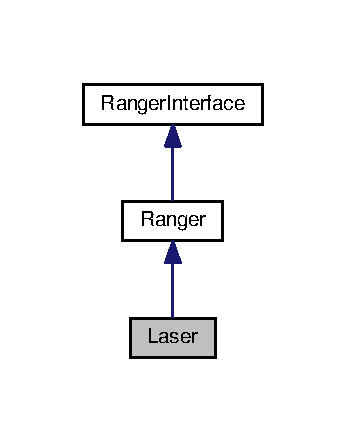
\includegraphics[width=166pt]{classLaser__inherit__graph}
\end{center}
\end{figure}


Collaboration diagram for Laser\+:\nopagebreak
\begin{figure}[H]
\begin{center}
\leavevmode
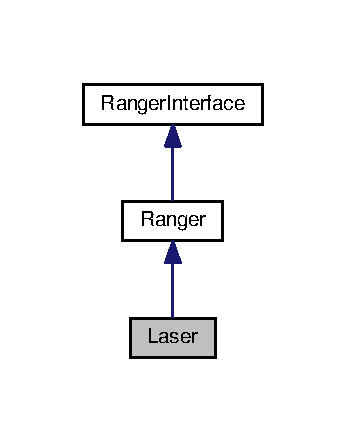
\includegraphics[width=166pt]{classLaser__coll__graph}
\end{center}
\end{figure}
\subsection*{Public Member Functions}
\begin{DoxyCompactItemize}
\item 
\hyperlink{classLaser_a68465e89283dffcc29a37e94693c6f87}{Laser} ()
\begin{DoxyCompactList}\small\item\em \hyperlink{classLaser}{Laser} default constructor. \end{DoxyCompactList}\item 
\hyperlink{classLaser_aa9baee5ed9775426e0b1d563c4687711}{$\sim$\+Laser} ()\hypertarget{classLaser_aa9baee5ed9775426e0b1d563c4687711}{}\label{classLaser_aa9baee5ed9775426e0b1d563c4687711}

\begin{DoxyCompactList}\small\item\em \hyperlink{classLaser}{Laser} default destructor. \end{DoxyCompactList}\end{DoxyCompactItemize}
\subsection*{Additional Inherited Members}


\subsection{Detailed Description}
The \hyperlink{classLaser}{Laser} class is a child class the \hyperlink{classRanger}{Ranger} Class. ~\newline
 This class creates lasers of sensing method type P\+O\+I\+NT. 

\begin{DoxyAuthor}{Author}
Ajal Singh 
\end{DoxyAuthor}
\begin{DoxyVersion}{Version}
1.\+0 
\end{DoxyVersion}
\begin{DoxyDate}{Date}
April 2020 
\end{DoxyDate}


\subsection{Constructor \& Destructor Documentation}
\index{Laser@{Laser}!Laser@{Laser}}
\index{Laser@{Laser}!Laser@{Laser}}
\subsubsection[{\texorpdfstring{Laser()}{Laser()}}]{\setlength{\rightskip}{0pt plus 5cm}Laser\+::\+Laser (
\begin{DoxyParamCaption}
{}
\end{DoxyParamCaption}
)}\hypertarget{classLaser_a68465e89283dffcc29a37e94693c6f87}{}\label{classLaser_a68465e89283dffcc29a37e94693c6f87}


\hyperlink{classLaser}{Laser} default constructor. 

Default constructor sets the fixed params. ~\newline
 set\+Model\+: \char`\"{}\+S\+I\+C\+K-\/\+X\+L\char`\"{} ~\newline
 set\+Field\+Of\+View\+: 180 degrees ~\newline
 set\+Sensing\+Method\+: P\+O\+I\+NT ~\newline
 set\+Angular\+Resolution\+: 10 degrees ~\newline
 set\+Max\+Range\+: 8 metres ~\newline
 set\+Min\+Range\+: 0.\+2 metres. 

The documentation for this class was generated from the following files\+:\begin{DoxyCompactItemize}
\item 
/home/ajal/git/pfms-\/2020a-\/ajalsingh/scratch/a2\+\_\+skeleton/\hyperlink{laser_8h}{laser.\+h}\item 
/home/ajal/git/pfms-\/2020a-\/ajalsingh/scratch/a2\+\_\+skeleton/laser.\+cpp\end{DoxyCompactItemize}

\hypertarget{structPoint}{}\section{Point Struct Reference}
\label{structPoint}\index{Point@{Point}}


The \hyperlink{structPoint}{Point} struct. Creates points with x and y coordinates.  




{\ttfamily \#include $<$rangerfusion.\+h$>$}

\subsection*{Public Attributes}
\begin{DoxyCompactItemize}
\item 
double \hyperlink{structPoint_ab99c56589bc8ad5fa5071387110a5bc7}{x}\hypertarget{structPoint_ab99c56589bc8ad5fa5071387110a5bc7}{}\label{structPoint_ab99c56589bc8ad5fa5071387110a5bc7}

\begin{DoxyCompactList}\small\item\em x coordinate \end{DoxyCompactList}\item 
double \hyperlink{structPoint_afa38be143ae800e6ad69ce8ed4df62d8}{y}\hypertarget{structPoint_afa38be143ae800e6ad69ce8ed4df62d8}{}\label{structPoint_afa38be143ae800e6ad69ce8ed4df62d8}

\begin{DoxyCompactList}\small\item\em y coordinate \end{DoxyCompactList}\end{DoxyCompactItemize}


\subsection{Detailed Description}
The \hyperlink{structPoint}{Point} struct. Creates points with x and y coordinates. 

The documentation for this struct was generated from the following file\+:\begin{DoxyCompactItemize}
\item 
/home/ajal/git/pfms-\/2020a-\/ajalsingh/scratch/a2\+\_\+skeleton/\hyperlink{rangerfusion_8h}{rangerfusion.\+h}\end{DoxyCompactItemize}

\hypertarget{classRanger}{}\section{Ranger Class Reference}
\label{classRanger}\index{Ranger@{Ranger}}


This class inherits methods from abstract class \hyperlink{classRangerInterface}{Ranger\+Interface} ~\newline
 This class is the base class to sensor classes (laser/sonar)  




{\ttfamily \#include $<$ranger.\+h$>$}



Inheritance diagram for Ranger\+:\nopagebreak
\begin{figure}[H]
\begin{center}
\leavevmode
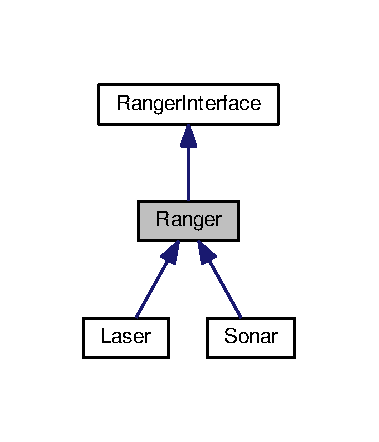
\includegraphics[width=182pt]{classRanger__inherit__graph}
\end{center}
\end{figure}


Collaboration diagram for Ranger\+:\nopagebreak
\begin{figure}[H]
\begin{center}
\leavevmode
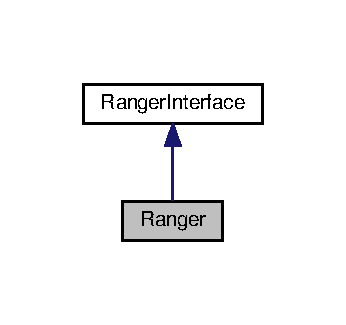
\includegraphics[width=166pt]{classRanger__coll__graph}
\end{center}
\end{figure}
\subsection*{Public Member Functions}
\begin{DoxyCompactItemize}
\item 
\hyperlink{classRanger_a65e1b9530f370b95cd673690c5bf02b5}{Ranger} ()
\begin{DoxyCompactList}\small\item\em \hyperlink{classRanger}{Ranger} default constructor. \end{DoxyCompactList}\item 
\hyperlink{classRanger_aba5e1cd17a61186c98fd026461682252}{$\sim$\+Ranger} ()\hypertarget{classRanger_aba5e1cd17a61186c98fd026461682252}{}\label{classRanger_aba5e1cd17a61186c98fd026461682252}

\begin{DoxyCompactList}\small\item\em \hyperlink{classRanger}{Ranger} default denstructor. \end{DoxyCompactList}\item 
std\+::vector$<$ double $>$ \hyperlink{classRanger_a2b76dc3e21da8a7abac830d09fa81241}{generate\+Data} ()
\begin{DoxyCompactList}\small\item\em Member function generates range data in metres for ranger objects. \end{DoxyCompactList}\item 
unsigned int \hyperlink{classRanger_a95b5013ae191d1e19b93fab002306718}{get\+Angular\+Resolution} (void)
\begin{DoxyCompactList}\small\item\em Member function gets Angular resolution in degrees for ranger. \end{DoxyCompactList}\item 
int \hyperlink{classRanger_a1c31d9a6c6a1c6ebd6325b36640b3576}{get\+Offset} (void)
\begin{DoxyCompactList}\small\item\em Member function gets Offset in degrees for ranger. \end{DoxyCompactList}\item 
unsigned int \hyperlink{classRanger_a4bca7dce56b7959257d90b1f30bf0271}{get\+Field\+Of\+View} (void)
\begin{DoxyCompactList}\small\item\em Member function gets Field of view for ranger in degrees anticlockwise. \end{DoxyCompactList}\item 
double \hyperlink{classRanger_aba5e81260e55089d9ff869051156a722}{get\+Max\+Range} (void)
\begin{DoxyCompactList}\small\item\em Member function gets max range in metres for ranger. \end{DoxyCompactList}\item 
double \hyperlink{classRanger_a646a06d3916179b9ebc4502bad169eec}{get\+Min\+Range} (void)
\begin{DoxyCompactList}\small\item\em Member function gets min range in metres for ranger. \end{DoxyCompactList}\item 
Sensing\+Method \hyperlink{classRanger_a2bcd122b3e549dc2525e04fa4dedc8ff}{get\+Sensing\+Method} (void)
\begin{DoxyCompactList}\small\item\em Member function gets Sensing Method of ranger. \end{DoxyCompactList}\item 
std\+::string \hyperlink{classRanger_a00c1e787c323b1e1aa28333059fc4db5}{get\+Model} (void)
\begin{DoxyCompactList}\small\item\em Member function gets Model code/number of ranger. \end{DoxyCompactList}\item 
int \hyperlink{classRanger_a03853a4887526a902a74bcb382b3827f}{get\+Num\+Samples} (void)
\begin{DoxyCompactList}\small\item\em Member function gets number of samples generated by ranger. \end{DoxyCompactList}\item 
bool \hyperlink{classRanger_abdf55e94ac5eea022f1ea229400f8f7c}{set\+Angular\+Resolution} (unsigned int angular\+\_\+resolution)
\begin{DoxyCompactList}\small\item\em Member function sets Angular Resolution of ranger in degrees. \end{DoxyCompactList}\item 
bool \hyperlink{classRanger_ae667f15d757a2c353ff8a2d0eed62055}{set\+Offset} (int offset)
\begin{DoxyCompactList}\small\item\em Member function sets offset of ranger in degrees anticlockwise. \end{DoxyCompactList}\end{DoxyCompactItemize}
\subsection*{Protected Member Functions}
\begin{DoxyCompactItemize}
\item 
void \hyperlink{classRanger_a5f76a88ea219e76ffa63d892fbcc70cb}{set\+Model} (std\+::string model)
\begin{DoxyCompactList}\small\item\em Member function sets Model code/number of ranger. \end{DoxyCompactList}\item 
bool \hyperlink{classRanger_a24876a4b461be9e61ba0c5e2df54d08f}{set\+Field\+Of\+View} (unsigned int field\+\_\+of\+\_\+view)
\begin{DoxyCompactList}\small\item\em Member function sets field of view of ranger in degrees. \end{DoxyCompactList}\item 
bool \hyperlink{classRanger_a4f288b0c2f0fca16b0ac2af14e91a0e1}{set\+Max\+Range} (double max\+\_\+range)
\begin{DoxyCompactList}\small\item\em Member function sets max range of ranger in metres. \end{DoxyCompactList}\item 
bool \hyperlink{classRanger_a8264b4a174d08df2bda42b70d1e45f22}{set\+Min\+Range} (double min\+\_\+range)
\begin{DoxyCompactList}\small\item\em Member function sets min range of ranger in metres. \end{DoxyCompactList}\item 
bool \hyperlink{classRanger_ae078104d1526fb6f1ab1c2e3a2b3d142}{set\+Sensing\+Method} (Sensing\+Method sensing\+\_\+method)
\begin{DoxyCompactList}\small\item\em Member function sets sensing method of ranger. \end{DoxyCompactList}\item 
bool \hyperlink{classRanger_a4f103e829a5fd74159f9c3f4d5fd3bf3}{set\+Num\+Samples} ()
\begin{DoxyCompactList}\small\item\em Member function sets number of samples generated by ranger. \end{DoxyCompactList}\end{DoxyCompactItemize}
\subsection*{Private Member Functions}
\begin{DoxyCompactItemize}
\item 
double \hyperlink{classRanger_ac2eb58a7ddd097583a46c3c6a1d30c8f}{get\+Random\+Number} (double \hyperlink{main_8cpp_a1447ad288a0a73454510f5777bdc3ed1}{seed})
\begin{DoxyCompactList}\small\item\em Member function generates a randoum double number using normal distribution. \end{DoxyCompactList}\end{DoxyCompactItemize}
\subsection*{Private Attributes}
\begin{DoxyCompactItemize}
\item 
std\+::vector$<$ double $>$ \hyperlink{classRanger_adef7fed47f032646f5023046de0bbc48}{data\+\_\+}
\begin{DoxyCompactList}\small\item\em Stores vector of random numbers/range. Size depends on ranger type. \end{DoxyCompactList}\item 
std\+::string \hyperlink{classRanger_a806db893039467e1f6f66335e8eabb7b}{model\+\_\+}\hypertarget{classRanger_a806db893039467e1f6f66335e8eabb7b}{}\label{classRanger_a806db893039467e1f6f66335e8eabb7b}

\begin{DoxyCompactList}\small\item\em Model code/number. \end{DoxyCompactList}\item 
int \hyperlink{classRanger_add17fe15ea0db50db1f678f9949cfc87}{offset\+\_\+}\hypertarget{classRanger_add17fe15ea0db50db1f678f9949cfc87}{}\label{classRanger_add17fe15ea0db50db1f678f9949cfc87}

\begin{DoxyCompactList}\small\item\em Offset. \end{DoxyCompactList}\item 
unsigned int \hyperlink{classRanger_a1f38aa37632d4b98adcdb772bc29a562}{field\+\_\+of\+\_\+view\+\_\+}\hypertarget{classRanger_a1f38aa37632d4b98adcdb772bc29a562}{}\label{classRanger_a1f38aa37632d4b98adcdb772bc29a562}

\begin{DoxyCompactList}\small\item\em Field of view. \end{DoxyCompactList}\item 
double \hyperlink{classRanger_aa2cc14d1f0d1110b63b4ac96d95610f1}{max\+\_\+range\+\_\+}\hypertarget{classRanger_aa2cc14d1f0d1110b63b4ac96d95610f1}{}\label{classRanger_aa2cc14d1f0d1110b63b4ac96d95610f1}

\begin{DoxyCompactList}\small\item\em Max Range. \end{DoxyCompactList}\item 
double \hyperlink{classRanger_a143fdd2a9b956ce61164d411bc8740b0}{min\+\_\+range\+\_\+}\hypertarget{classRanger_a143fdd2a9b956ce61164d411bc8740b0}{}\label{classRanger_a143fdd2a9b956ce61164d411bc8740b0}

\begin{DoxyCompactList}\small\item\em Min Range. \end{DoxyCompactList}\item 
Sensing\+Method \hyperlink{classRanger_a2d81156691f120f123ea3ab6e3028ef1}{sensing\+\_\+method\+\_\+}\hypertarget{classRanger_a2d81156691f120f123ea3ab6e3028ef1}{}\label{classRanger_a2d81156691f120f123ea3ab6e3028ef1}

\begin{DoxyCompactList}\small\item\em Sensing method, i.\+e. type of sensor (P\+O\+I\+NT or C\+O\+NE) \end{DoxyCompactList}\item 
unsigned int \hyperlink{classRanger_af3ee97c4a20ab9a831ea7c87eb85a5b0}{number\+\_\+of\+\_\+samples\+\_\+}\hypertarget{classRanger_af3ee97c4a20ab9a831ea7c87eb85a5b0}{}\label{classRanger_af3ee97c4a20ab9a831ea7c87eb85a5b0}

\begin{DoxyCompactList}\small\item\em Number of data samples generated by a sensor. \end{DoxyCompactList}\item 
unsigned int \hyperlink{classRanger_a0f8dec4bca07df9c2154c7746fd25e77}{angular\+\_\+resolution\+\_\+}\hypertarget{classRanger_a0f8dec4bca07df9c2154c7746fd25e77}{}\label{classRanger_a0f8dec4bca07df9c2154c7746fd25e77}

\begin{DoxyCompactList}\small\item\em Angular resultion. \end{DoxyCompactList}\end{DoxyCompactItemize}


\subsection{Detailed Description}
This class inherits methods from abstract class \hyperlink{classRangerInterface}{Ranger\+Interface} ~\newline
 This class is the base class to sensor classes (laser/sonar) 

\begin{DoxyAuthor}{Author}
Ajal Singh 
\end{DoxyAuthor}
\begin{DoxyVersion}{Version}
1.\+0 
\end{DoxyVersion}
\begin{DoxyDate}{Date}
April 2020 
\end{DoxyDate}


\subsection{Constructor \& Destructor Documentation}
\index{Ranger@{Ranger}!Ranger@{Ranger}}
\index{Ranger@{Ranger}!Ranger@{Ranger}}
\subsubsection[{\texorpdfstring{Ranger()}{Ranger()}}]{\setlength{\rightskip}{0pt plus 5cm}Ranger\+::\+Ranger (
\begin{DoxyParamCaption}
{}
\end{DoxyParamCaption}
)}\hypertarget{classRanger_a65e1b9530f370b95cd673690c5bf02b5}{}\label{classRanger_a65e1b9530f370b95cd673690c5bf02b5}


\hyperlink{classRanger}{Ranger} default constructor. 

Default constructor sets the offset to 0 and sets model to \char`\"{}unknown\char`\"{}. 

\subsection{Member Function Documentation}
\index{Ranger@{Ranger}!generate\+Data@{generate\+Data}}
\index{generate\+Data@{generate\+Data}!Ranger@{Ranger}}
\subsubsection[{\texorpdfstring{generate\+Data()}{generateData()}}]{\setlength{\rightskip}{0pt plus 5cm}std\+::vector$<$ double $>$ Ranger\+::generate\+Data (
\begin{DoxyParamCaption}
{}
\end{DoxyParamCaption}
)\hspace{0.3cm}{\ttfamily [virtual]}}\hypertarget{classRanger_a2b76dc3e21da8a7abac830d09fa81241}{}\label{classRanger_a2b76dc3e21da8a7abac830d09fa81241}


Member function generates range data in metres for ranger objects. 

\begin{DoxyReturn}{Returns}
Vector of ranges
\end{DoxyReturn}
Generates random range values within max and min limits. ~\newline
 Number of values generated is equal to the number of samples. 

Implements \hyperlink{classRangerInterface}{Ranger\+Interface}.

\index{Ranger@{Ranger}!get\+Angular\+Resolution@{get\+Angular\+Resolution}}
\index{get\+Angular\+Resolution@{get\+Angular\+Resolution}!Ranger@{Ranger}}
\subsubsection[{\texorpdfstring{get\+Angular\+Resolution(void)}{getAngularResolution(void)}}]{\setlength{\rightskip}{0pt plus 5cm}unsigned int Ranger\+::get\+Angular\+Resolution (
\begin{DoxyParamCaption}
\item[{void}]{}
\end{DoxyParamCaption}
)\hspace{0.3cm}{\ttfamily [virtual]}}\hypertarget{classRanger_a95b5013ae191d1e19b93fab002306718}{}\label{classRanger_a95b5013ae191d1e19b93fab002306718}


Member function gets Angular resolution in degrees for ranger. 

\begin{DoxyReturn}{Returns}
Angular Resolution 
\end{DoxyReturn}


Implements \hyperlink{classRangerInterface}{Ranger\+Interface}.

\index{Ranger@{Ranger}!get\+Field\+Of\+View@{get\+Field\+Of\+View}}
\index{get\+Field\+Of\+View@{get\+Field\+Of\+View}!Ranger@{Ranger}}
\subsubsection[{\texorpdfstring{get\+Field\+Of\+View(void)}{getFieldOfView(void)}}]{\setlength{\rightskip}{0pt plus 5cm}unsigned int Ranger\+::get\+Field\+Of\+View (
\begin{DoxyParamCaption}
\item[{void}]{}
\end{DoxyParamCaption}
)\hspace{0.3cm}{\ttfamily [virtual]}}\hypertarget{classRanger_a4bca7dce56b7959257d90b1f30bf0271}{}\label{classRanger_a4bca7dce56b7959257d90b1f30bf0271}


Member function gets Field of view for ranger in degrees anticlockwise. 

\begin{DoxyReturn}{Returns}
F\+OV 
\end{DoxyReturn}


Implements \hyperlink{classRangerInterface}{Ranger\+Interface}.

\index{Ranger@{Ranger}!get\+Max\+Range@{get\+Max\+Range}}
\index{get\+Max\+Range@{get\+Max\+Range}!Ranger@{Ranger}}
\subsubsection[{\texorpdfstring{get\+Max\+Range(void)}{getMaxRange(void)}}]{\setlength{\rightskip}{0pt plus 5cm}double Ranger\+::get\+Max\+Range (
\begin{DoxyParamCaption}
\item[{void}]{}
\end{DoxyParamCaption}
)\hspace{0.3cm}{\ttfamily [virtual]}}\hypertarget{classRanger_aba5e81260e55089d9ff869051156a722}{}\label{classRanger_aba5e81260e55089d9ff869051156a722}


Member function gets max range in metres for ranger. 

\begin{DoxyReturn}{Returns}
Max range 
\end{DoxyReturn}


Implements \hyperlink{classRangerInterface}{Ranger\+Interface}.

\index{Ranger@{Ranger}!get\+Min\+Range@{get\+Min\+Range}}
\index{get\+Min\+Range@{get\+Min\+Range}!Ranger@{Ranger}}
\subsubsection[{\texorpdfstring{get\+Min\+Range(void)}{getMinRange(void)}}]{\setlength{\rightskip}{0pt plus 5cm}double Ranger\+::get\+Min\+Range (
\begin{DoxyParamCaption}
\item[{void}]{}
\end{DoxyParamCaption}
)\hspace{0.3cm}{\ttfamily [virtual]}}\hypertarget{classRanger_a646a06d3916179b9ebc4502bad169eec}{}\label{classRanger_a646a06d3916179b9ebc4502bad169eec}


Member function gets min range in metres for ranger. 

\begin{DoxyReturn}{Returns}
Min range 
\end{DoxyReturn}


Implements \hyperlink{classRangerInterface}{Ranger\+Interface}.

\index{Ranger@{Ranger}!get\+Model@{get\+Model}}
\index{get\+Model@{get\+Model}!Ranger@{Ranger}}
\subsubsection[{\texorpdfstring{get\+Model(void)}{getModel(void)}}]{\setlength{\rightskip}{0pt plus 5cm}std\+::string Ranger\+::get\+Model (
\begin{DoxyParamCaption}
\item[{void}]{}
\end{DoxyParamCaption}
)}\hypertarget{classRanger_a00c1e787c323b1e1aa28333059fc4db5}{}\label{classRanger_a00c1e787c323b1e1aa28333059fc4db5}


Member function gets Model code/number of ranger. 

\begin{DoxyReturn}{Returns}
Model code/number 
\end{DoxyReturn}
\index{Ranger@{Ranger}!get\+Num\+Samples@{get\+Num\+Samples}}
\index{get\+Num\+Samples@{get\+Num\+Samples}!Ranger@{Ranger}}
\subsubsection[{\texorpdfstring{get\+Num\+Samples(void)}{getNumSamples(void)}}]{\setlength{\rightskip}{0pt plus 5cm}int Ranger\+::get\+Num\+Samples (
\begin{DoxyParamCaption}
\item[{void}]{}
\end{DoxyParamCaption}
)}\hypertarget{classRanger_a03853a4887526a902a74bcb382b3827f}{}\label{classRanger_a03853a4887526a902a74bcb382b3827f}


Member function gets number of samples generated by ranger. 

\begin{DoxyReturn}{Returns}
Number of samples 
\end{DoxyReturn}
\index{Ranger@{Ranger}!get\+Offset@{get\+Offset}}
\index{get\+Offset@{get\+Offset}!Ranger@{Ranger}}
\subsubsection[{\texorpdfstring{get\+Offset(void)}{getOffset(void)}}]{\setlength{\rightskip}{0pt plus 5cm}int Ranger\+::get\+Offset (
\begin{DoxyParamCaption}
\item[{void}]{}
\end{DoxyParamCaption}
)\hspace{0.3cm}{\ttfamily [virtual]}}\hypertarget{classRanger_a1c31d9a6c6a1c6ebd6325b36640b3576}{}\label{classRanger_a1c31d9a6c6a1c6ebd6325b36640b3576}


Member function gets Offset in degrees for ranger. 

\begin{DoxyReturn}{Returns}
Offset 
\end{DoxyReturn}


Implements \hyperlink{classRangerInterface}{Ranger\+Interface}.

\index{Ranger@{Ranger}!get\+Random\+Number@{get\+Random\+Number}}
\index{get\+Random\+Number@{get\+Random\+Number}!Ranger@{Ranger}}
\subsubsection[{\texorpdfstring{get\+Random\+Number(double seed)}{getRandomNumber(double seed)}}]{\setlength{\rightskip}{0pt plus 5cm}double Ranger\+::get\+Random\+Number (
\begin{DoxyParamCaption}
\item[{double}]{seed}
\end{DoxyParamCaption}
)\hspace{0.3cm}{\ttfamily [private]}}\hypertarget{classRanger_ac2eb58a7ddd097583a46c3c6a1d30c8f}{}\label{classRanger_ac2eb58a7ddd097583a46c3c6a1d30c8f}


Member function generates a randoum double number using normal distribution. 


\begin{DoxyParams}{Parameters}
{\em seed} & \\
\hline
\end{DoxyParams}
\begin{DoxyReturn}{Returns}
Random number 
\end{DoxyReturn}
\index{Ranger@{Ranger}!get\+Sensing\+Method@{get\+Sensing\+Method}}
\index{get\+Sensing\+Method@{get\+Sensing\+Method}!Ranger@{Ranger}}
\subsubsection[{\texorpdfstring{get\+Sensing\+Method(void)}{getSensingMethod(void)}}]{\setlength{\rightskip}{0pt plus 5cm}Sensing\+Method Ranger\+::get\+Sensing\+Method (
\begin{DoxyParamCaption}
\item[{void}]{}
\end{DoxyParamCaption}
)\hspace{0.3cm}{\ttfamily [virtual]}}\hypertarget{classRanger_a2bcd122b3e549dc2525e04fa4dedc8ff}{}\label{classRanger_a2bcd122b3e549dc2525e04fa4dedc8ff}


Member function gets Sensing Method of ranger. 

\begin{DoxyReturn}{Returns}
Sensing method 
\end{DoxyReturn}
\begin{DoxySeeAlso}{See also}
\hyperlink{classRanger}{Ranger} Interface class Sensing\+Method enum 
\end{DoxySeeAlso}


Implements \hyperlink{classRangerInterface}{Ranger\+Interface}.

\index{Ranger@{Ranger}!set\+Angular\+Resolution@{set\+Angular\+Resolution}}
\index{set\+Angular\+Resolution@{set\+Angular\+Resolution}!Ranger@{Ranger}}
\subsubsection[{\texorpdfstring{set\+Angular\+Resolution(unsigned int angular\+\_\+resolution)}{setAngularResolution(unsigned int angular_resolution)}}]{\setlength{\rightskip}{0pt plus 5cm}bool Ranger\+::set\+Angular\+Resolution (
\begin{DoxyParamCaption}
\item[{unsigned int}]{angular\+\_\+resolution}
\end{DoxyParamCaption}
)\hspace{0.3cm}{\ttfamily [virtual]}}\hypertarget{classRanger_abdf55e94ac5eea022f1ea229400f8f7c}{}\label{classRanger_abdf55e94ac5eea022f1ea229400f8f7c}


Member function sets Angular Resolution of ranger in degrees. 


\begin{DoxyParams}{Parameters}
{\em angular\+\_\+resolution} & \\
\hline
\end{DoxyParams}
\begin{DoxyReturn}{Returns}
True if param set successfully, otherwise false
\end{DoxyReturn}
Sets angular resolution according to \hyperlink{classRanger}{Ranger}\textquotesingle{}s Sensing\+Method type. \begin{DoxyNote}{Note}
for P\+O\+I\+NT type, 10 and 30 are the only acceptable values. ~\newline
 for C\+O\+NE type, angular velocity will be equal to field of view. ~\newline
 All other values will return false. 
\end{DoxyNote}


Implements \hyperlink{classRangerInterface}{Ranger\+Interface}.

\index{Ranger@{Ranger}!set\+Field\+Of\+View@{set\+Field\+Of\+View}}
\index{set\+Field\+Of\+View@{set\+Field\+Of\+View}!Ranger@{Ranger}}
\subsubsection[{\texorpdfstring{set\+Field\+Of\+View(unsigned int field\+\_\+of\+\_\+view)}{setFieldOfView(unsigned int field_of_view)}}]{\setlength{\rightskip}{0pt plus 5cm}bool Ranger\+::set\+Field\+Of\+View (
\begin{DoxyParamCaption}
\item[{unsigned int}]{field\+\_\+of\+\_\+view}
\end{DoxyParamCaption}
)\hspace{0.3cm}{\ttfamily [protected]}, {\ttfamily [virtual]}}\hypertarget{classRanger_a24876a4b461be9e61ba0c5e2df54d08f}{}\label{classRanger_a24876a4b461be9e61ba0c5e2df54d08f}


Member function sets field of view of ranger in degrees. 


\begin{DoxyParams}{Parameters}
{\em field\+\_\+of\+\_\+view} & \\
\hline
\end{DoxyParams}
\begin{DoxyReturn}{Returns}
True if param set successfully, otherwise false 
\end{DoxyReturn}


Implements \hyperlink{classRangerInterface}{Ranger\+Interface}.

\index{Ranger@{Ranger}!set\+Max\+Range@{set\+Max\+Range}}
\index{set\+Max\+Range@{set\+Max\+Range}!Ranger@{Ranger}}
\subsubsection[{\texorpdfstring{set\+Max\+Range(double max\+\_\+range)}{setMaxRange(double max_range)}}]{\setlength{\rightskip}{0pt plus 5cm}bool Ranger\+::set\+Max\+Range (
\begin{DoxyParamCaption}
\item[{double}]{max\+\_\+range}
\end{DoxyParamCaption}
)\hspace{0.3cm}{\ttfamily [protected]}}\hypertarget{classRanger_a4f288b0c2f0fca16b0ac2af14e91a0e1}{}\label{classRanger_a4f288b0c2f0fca16b0ac2af14e91a0e1}


Member function sets max range of ranger in metres. 


\begin{DoxyParams}{Parameters}
{\em max\+\_\+range} & \\
\hline
\end{DoxyParams}
\begin{DoxyReturn}{Returns}
True if param set successfully, otherwise false 
\end{DoxyReturn}
\index{Ranger@{Ranger}!set\+Min\+Range@{set\+Min\+Range}}
\index{set\+Min\+Range@{set\+Min\+Range}!Ranger@{Ranger}}
\subsubsection[{\texorpdfstring{set\+Min\+Range(double min\+\_\+range)}{setMinRange(double min_range)}}]{\setlength{\rightskip}{0pt plus 5cm}bool Ranger\+::set\+Min\+Range (
\begin{DoxyParamCaption}
\item[{double}]{min\+\_\+range}
\end{DoxyParamCaption}
)\hspace{0.3cm}{\ttfamily [protected]}}\hypertarget{classRanger_a8264b4a174d08df2bda42b70d1e45f22}{}\label{classRanger_a8264b4a174d08df2bda42b70d1e45f22}


Member function sets min range of ranger in metres. 


\begin{DoxyParams}{Parameters}
{\em min\+\_\+range} & \\
\hline
\end{DoxyParams}
\begin{DoxyReturn}{Returns}
True if param set successfully, otherwise false 
\end{DoxyReturn}
\index{Ranger@{Ranger}!set\+Model@{set\+Model}}
\index{set\+Model@{set\+Model}!Ranger@{Ranger}}
\subsubsection[{\texorpdfstring{set\+Model(std\+::string model)}{setModel(std::string model)}}]{\setlength{\rightskip}{0pt plus 5cm}void Ranger\+::set\+Model (
\begin{DoxyParamCaption}
\item[{std\+::string}]{model}
\end{DoxyParamCaption}
)\hspace{0.3cm}{\ttfamily [protected]}}\hypertarget{classRanger_a5f76a88ea219e76ffa63d892fbcc70cb}{}\label{classRanger_a5f76a88ea219e76ffa63d892fbcc70cb}


Member function sets Model code/number of ranger. 

\begin{DoxyReturn}{Returns}
model code/number 
\end{DoxyReturn}
\index{Ranger@{Ranger}!set\+Num\+Samples@{set\+Num\+Samples}}
\index{set\+Num\+Samples@{set\+Num\+Samples}!Ranger@{Ranger}}
\subsubsection[{\texorpdfstring{set\+Num\+Samples()}{setNumSamples()}}]{\setlength{\rightskip}{0pt plus 5cm}bool Ranger\+::set\+Num\+Samples (
\begin{DoxyParamCaption}
{}
\end{DoxyParamCaption}
)\hspace{0.3cm}{\ttfamily [protected]}}\hypertarget{classRanger_a4f103e829a5fd74159f9c3f4d5fd3bf3}{}\label{classRanger_a4f103e829a5fd74159f9c3f4d5fd3bf3}


Member function sets number of samples generated by ranger. 

\begin{DoxyReturn}{Returns}
True if param set successfully, otherwise false
\end{DoxyReturn}
Number of samples for P\+O\+I\+NT type is influenced by field of view and angular resolution. ~\newline
 Number of samples for C\+O\+NE type is 1 \begin{DoxyNote}{Note}
This method is automatically called after angualar resolution is set 
\end{DoxyNote}
\index{Ranger@{Ranger}!set\+Offset@{set\+Offset}}
\index{set\+Offset@{set\+Offset}!Ranger@{Ranger}}
\subsubsection[{\texorpdfstring{set\+Offset(int offset)}{setOffset(int offset)}}]{\setlength{\rightskip}{0pt plus 5cm}bool Ranger\+::set\+Offset (
\begin{DoxyParamCaption}
\item[{int}]{offset}
\end{DoxyParamCaption}
)\hspace{0.3cm}{\ttfamily [virtual]}}\hypertarget{classRanger_ae667f15d757a2c353ff8a2d0eed62055}{}\label{classRanger_ae667f15d757a2c353ff8a2d0eed62055}


Member function sets offset of ranger in degrees anticlockwise. 


\begin{DoxyParams}{Parameters}
{\em offset} & \\
\hline
\end{DoxyParams}
\begin{DoxyReturn}{Returns}
True if param set successfully, otherwise false
\end{DoxyReturn}
\begin{DoxyNote}{Note}
-\/180 $<$= offset $<$= 180 degrees. Values out of range will return false. 
\end{DoxyNote}


Implements \hyperlink{classRangerInterface}{Ranger\+Interface}.

\index{Ranger@{Ranger}!set\+Sensing\+Method@{set\+Sensing\+Method}}
\index{set\+Sensing\+Method@{set\+Sensing\+Method}!Ranger@{Ranger}}
\subsubsection[{\texorpdfstring{set\+Sensing\+Method(\+Sensing\+Method sensing\+\_\+method)}{setSensingMethod(SensingMethod sensing_method)}}]{\setlength{\rightskip}{0pt plus 5cm}bool Ranger\+::set\+Sensing\+Method (
\begin{DoxyParamCaption}
\item[{Sensing\+Method}]{sensing\+\_\+method}
\end{DoxyParamCaption}
)\hspace{0.3cm}{\ttfamily [protected]}}\hypertarget{classRanger_ae078104d1526fb6f1ab1c2e3a2b3d142}{}\label{classRanger_ae078104d1526fb6f1ab1c2e3a2b3d142}


Member function sets sensing method of ranger. 


\begin{DoxyParams}{Parameters}
{\em sensing\+\_\+method} & \\
\hline
\end{DoxyParams}
\begin{DoxyReturn}{Returns}
True if param set successfully, otherwise false 
\end{DoxyReturn}
\begin{DoxySeeAlso}{See also}
\hyperlink{classRanger}{Ranger} Interface class Sensing\+Method enum 
\end{DoxySeeAlso}


\subsection{Member Data Documentation}
\index{Ranger@{Ranger}!data\+\_\+@{data\+\_\+}}
\index{data\+\_\+@{data\+\_\+}!Ranger@{Ranger}}
\subsubsection[{\texorpdfstring{data\+\_\+}{data_}}]{\setlength{\rightskip}{0pt plus 5cm}std\+::vector$<$double$>$ Ranger\+::data\+\_\+\hspace{0.3cm}{\ttfamily [private]}}\hypertarget{classRanger_adef7fed47f032646f5023046de0bbc48}{}\label{classRanger_adef7fed47f032646f5023046de0bbc48}


Stores vector of random numbers/range. Size depends on ranger type. 

ranger parameters 

The documentation for this class was generated from the following files\+:\begin{DoxyCompactItemize}
\item 
/home/ajal/git/pfms-\/2020a-\/ajalsingh/scratch/a2\+\_\+skeleton/\hyperlink{ranger_8h}{ranger.\+h}\item 
/home/ajal/git/pfms-\/2020a-\/ajalsingh/scratch/a2\+\_\+skeleton/ranger.\+cpp\end{DoxyCompactItemize}

\hypertarget{classRangerFusion}{}\section{Ranger\+Fusion Class Reference}
\label{classRangerFusion}\index{Ranger\+Fusion@{Ranger\+Fusion}}


The \hyperlink{classRangerFusion}{Ranger\+Fusion} class is a child of abstract class \hyperlink{classRangerFusionInterface}{Ranger\+Fusion\+Interface} Accepts cells and rangers and fuses the data. Checks if the ranger data occupies a cell, or passes through the cell (free). \hyperlink{classCell}{Cell} state is then updated.  




{\ttfamily \#include $<$rangerfusion.\+h$>$}



Inheritance diagram for Ranger\+Fusion\+:\nopagebreak
\begin{figure}[H]
\begin{center}
\leavevmode
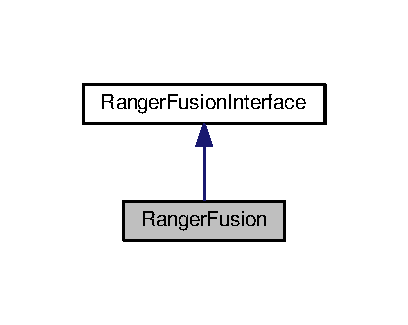
\includegraphics[width=196pt]{classRangerFusion__inherit__graph}
\end{center}
\end{figure}


Collaboration diagram for Ranger\+Fusion\+:\nopagebreak
\begin{figure}[H]
\begin{center}
\leavevmode
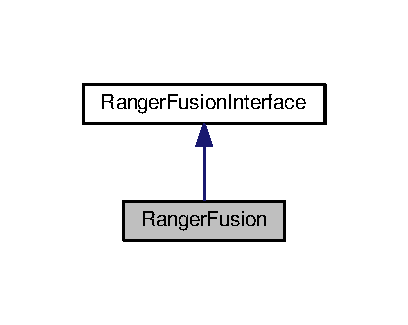
\includegraphics[width=196pt]{classRangerFusion__coll__graph}
\end{center}
\end{figure}
\subsection*{Public Member Functions}
\begin{DoxyCompactItemize}
\item 
\hyperlink{classRangerFusion_ab09391c929404c32ad3e2cb7ab1d38bc}{Ranger\+Fusion} ()\hypertarget{classRangerFusion_ab09391c929404c32ad3e2cb7ab1d38bc}{}\label{classRangerFusion_ab09391c929404c32ad3e2cb7ab1d38bc}

\begin{DoxyCompactList}\small\item\em \hyperlink{classRangerFusion}{Ranger\+Fusion} default constructor. \end{DoxyCompactList}\item 
\hyperlink{classRangerFusion_a25fd5aaa541efc80c5251bc9be903379}{$\sim$\+Ranger\+Fusion} ()\hypertarget{classRangerFusion_a25fd5aaa541efc80c5251bc9be903379}{}\label{classRangerFusion_a25fd5aaa541efc80c5251bc9be903379}

\begin{DoxyCompactList}\small\item\em \hyperlink{classRangerFusion}{Ranger\+Fusion} default destructor. \end{DoxyCompactList}\item 
void \hyperlink{classRangerFusion_a01909c08b2a974e68b031056db730aba}{set\+Rangers} (std\+::vector$<$ \hyperlink{classRangerInterface}{Ranger\+Interface} $\ast$ $>$ rangers)
\begin{DoxyCompactList}\small\item\em Member function prepares ranger data for fusion. \end{DoxyCompactList}\item 
void \hyperlink{classRangerFusion_ae3128f8cc8f4cb955d8db661aefba3dc}{set\+Cells} (std\+::vector$<$ \hyperlink{classCell}{Cell} $\ast$ $>$ cells)
\begin{DoxyCompactList}\small\item\em Member function prepares cells data for fusion. \end{DoxyCompactList}\item 
void \hyperlink{classRangerFusion_aa9265f72bc3572567c9cf98cf6d9f0e1}{grab\+And\+Fuse\+Data} ()\hypertarget{classRangerFusion_aa9265f72bc3572567c9cf98cf6d9f0e1}{}\label{classRangerFusion_aa9265f72bc3572567c9cf98cf6d9f0e1}

\begin{DoxyCompactList}\small\item\em Member function checks if the ranger data occupies a cell, or passes through the cell (free). \hyperlink{classCell}{Cell} state is then updated, O\+C\+C\+U\+P\+I\+ED (-\/1), F\+R\+EE (1), and U\+N\+K\+N\+O\+W\+N(0) \end{DoxyCompactList}\item 
std\+::vector$<$ std\+::vector$<$ double $>$ $>$ \hyperlink{classRangerFusion_a5780383fdffe121a7a2372a047819ba9}{get\+Raw\+Range\+Data} ()
\begin{DoxyCompactList}\small\item\em Member function gets raw range data generated from ranger class which was used in fusion. \end{DoxyCompactList}\item 
std\+::vector$<$ \hyperlink{classCell}{Cell} $\ast$ $>$ \hyperlink{classRangerFusion_ad50617885caf58465966d9a6c9c56713}{get\+Cells} (void)
\begin{DoxyCompactList}\small\item\em Member function gets cells with updated cell states after fusion. \end{DoxyCompactList}\end{DoxyCompactItemize}
\subsection*{Private Member Functions}
\begin{DoxyCompactItemize}
\item 
void \hyperlink{classRangerFusion_a5f2963a4d53c84e5ba293a25fd67fb2f}{calculate\+Cell\+Geometry} (\hyperlink{classCell}{Cell} $\ast$cell)
\begin{DoxyCompactList}\small\item\em Member function calculates \hyperlink{classCell}{Cell} Geometry. \end{DoxyCompactList}\item 
int \hyperlink{classRangerFusion_afa8523c62b05aa5d6d5fa2bf22d7219d}{analyse\+Laser} (double data\+\_\+x, double data\+\_\+y)
\begin{DoxyCompactList}\small\item\em Member function checks if the laser point provided, has any interaction with cell. \end{DoxyCompactList}\item 
int \hyperlink{classRangerFusion_a18d2a54f882b09d9041c952f957e324c}{analyse\+Sonar} (\hyperlink{structPoint}{Point} sonar\+\_\+p1, \hyperlink{structPoint}{Point} sonar\+\_\+p2)
\begin{DoxyCompactList}\small\item\em Member function checks if the sonar data provided, has any interaction with cell. \end{DoxyCompactList}\item 
bool \hyperlink{classRangerFusion_a16257a2c9e7e482de25bc8a0968c2e70}{check\+For\+Intersect} (\hyperlink{structPoint}{Point} p1, \hyperlink{structPoint}{Point} p2, \hyperlink{structPoint}{Point} p3, \hyperlink{structPoint}{Point} p4)
\begin{DoxyCompactList}\small\item\em Member function checks if two given lines intersect. \end{DoxyCompactList}\item 
double \hyperlink{classRangerFusion_af73b5c54aacf13aea39e2f18916b6608}{orientation} (\hyperlink{structPoint}{Point} p, \hyperlink{structPoint}{Point} q, \hyperlink{structPoint}{Point} r)
\begin{DoxyCompactList}\small\item\em Member function determines the orientation of ordered triplet (p,q,r) \end{DoxyCompactList}\item 
bool \hyperlink{classRangerFusion_a3acbc5680a1ae726bdff3ca84ae84d09}{check\+On\+Segment} (\hyperlink{structPoint}{Point} p, \hyperlink{structPoint}{Point} q, \hyperlink{structPoint}{Point} r)
\begin{DoxyCompactList}\small\item\em Member function given three colinear points p, q, r, the function checks if point q lies on line segment \textquotesingle{}pr\textquotesingle{}. \end{DoxyCompactList}\item 
double \hyperlink{classRangerFusion_a358e04e31466f1ba5daa20d1de38ff9b}{triangle\+Area} (\hyperlink{structPoint}{Point} p1, \hyperlink{structPoint}{Point} p2, \hyperlink{structPoint}{Point} p3)
\begin{DoxyCompactList}\small\item\em Member function calculates area of triangle formed by \hyperlink{structPoint}{Point} p1, \hyperlink{structPoint}{Point} p2, and \hyperlink{structPoint}{Point} p3. \end{DoxyCompactList}\end{DoxyCompactItemize}
\subsection*{Private Attributes}
\begin{DoxyCompactItemize}
\item 
std\+::vector$<$ std\+::vector$<$ double $>$ $>$ \hyperlink{classRangerFusion_a2fa4a5228da72e2f33dd1121cf2644a7}{data\+\_\+}\hypertarget{classRangerFusion_a2fa4a5228da72e2f33dd1121cf2644a7}{}\label{classRangerFusion_a2fa4a5228da72e2f33dd1121cf2644a7}

\begin{DoxyCompactList}\small\item\em Holds raw ranger data. \end{DoxyCompactList}\item 
std\+::vector$<$ \hyperlink{classRangerInterface}{Ranger\+Interface} $\ast$ $>$ \hyperlink{classRangerFusion_ac0608d2ac2fbccdd394f3e920d2f4db9}{rangers\+\_\+}\hypertarget{classRangerFusion_ac0608d2ac2fbccdd394f3e920d2f4db9}{}\label{classRangerFusion_ac0608d2ac2fbccdd394f3e920d2f4db9}

\begin{DoxyCompactList}\small\item\em \hyperlink{classRangerInterface}{Ranger\+Interface} Class object pointers. \end{DoxyCompactList}\item 
std\+::vector$<$ \hyperlink{classCell}{Cell} $\ast$ $>$ \hyperlink{classRangerFusion_aafc6b84823abfae3dc3a5095da43888e}{cells\+\_\+}\hypertarget{classRangerFusion_aafc6b84823abfae3dc3a5095da43888e}{}\label{classRangerFusion_aafc6b84823abfae3dc3a5095da43888e}

\begin{DoxyCompactList}\small\item\em \hyperlink{classCell}{Cell} class object pointers. \end{DoxyCompactList}\item 
std\+::vector$<$ std\+::vector$<$ double $>$ $>$ \hyperlink{classRangerFusion_a2e57dd1467e95392d4652230279ea189}{angle\+\_\+for\+\_\+fusion\+\_\+}
\begin{DoxyCompactList}\small\item\em Holds generated data of rangers. ~\newline
 Every even element (0,2,...) holds a vector of angles. \end{DoxyCompactList}\item 
std\+::vector$<$ double $>$ \hyperlink{classRangerFusion_ae250d57e1fc380c5a07bceabb75561fa}{cell\+\_\+side\+\_\+coordinates\+\_\+}\hypertarget{classRangerFusion_ae250d57e1fc380c5a07bceabb75561fa}{}\label{classRangerFusion_ae250d57e1fc380c5a07bceabb75561fa}

\begin{DoxyCompactList}\small\item\em Holds upper and lower boundaries (x and y) of a cell. \end{DoxyCompactList}\item 
std\+::vector$<$ \hyperlink{structPoint}{Point} $>$ \hyperlink{classRangerFusion_a87b7d6ab48ffa42bf845f24ffc8f38cd}{cell\+\_\+points\+\_\+}\hypertarget{classRangerFusion_a87b7d6ab48ffa42bf845f24ffc8f38cd}{}\label{classRangerFusion_a87b7d6ab48ffa42bf845f24ffc8f38cd}

\begin{DoxyCompactList}\small\item\em Holds the four corners of a cell as points. \end{DoxyCompactList}\end{DoxyCompactItemize}


\subsection{Detailed Description}
The \hyperlink{classRangerFusion}{Ranger\+Fusion} class is a child of abstract class \hyperlink{classRangerFusionInterface}{Ranger\+Fusion\+Interface} Accepts cells and rangers and fuses the data. Checks if the ranger data occupies a cell, or passes through the cell (free). \hyperlink{classCell}{Cell} state is then updated. 

\subsection{Member Function Documentation}
\index{Ranger\+Fusion@{Ranger\+Fusion}!analyse\+Laser@{analyse\+Laser}}
\index{analyse\+Laser@{analyse\+Laser}!Ranger\+Fusion@{Ranger\+Fusion}}
\subsubsection[{\texorpdfstring{analyse\+Laser(double data\+\_\+x, double data\+\_\+y)}{analyseLaser(double data_x, double data_y)}}]{\setlength{\rightskip}{0pt plus 5cm}int Ranger\+Fusion\+::analyse\+Laser (
\begin{DoxyParamCaption}
\item[{double}]{data\+\_\+x, }
\item[{double}]{data\+\_\+y}
\end{DoxyParamCaption}
)\hspace{0.3cm}{\ttfamily [private]}}\hypertarget{classRangerFusion_afa8523c62b05aa5d6d5fa2bf22d7219d}{}\label{classRangerFusion_afa8523c62b05aa5d6d5fa2bf22d7219d}


Member function checks if the laser point provided, has any interaction with cell. 


\begin{DoxyParams}{Parameters}
{\em data\+\_\+x} & x coordinate of laser data point \\
\hline
{\em data\+\_\+y} & y of laser data point \\
\hline
\end{DoxyParams}
\begin{DoxyReturn}{Returns}
O\+C\+C\+U\+P\+I\+ED\+: -\/1 ~\newline
 F\+R\+EE\+: 1 (\hyperlink{classLaser}{Laser} passes through cell) ~\newline
 U\+N\+K\+N\+O\+WN\+: 0 
\end{DoxyReturn}
\index{Ranger\+Fusion@{Ranger\+Fusion}!analyse\+Sonar@{analyse\+Sonar}}
\index{analyse\+Sonar@{analyse\+Sonar}!Ranger\+Fusion@{Ranger\+Fusion}}
\subsubsection[{\texorpdfstring{analyse\+Sonar(\+Point sonar\+\_\+p1, Point sonar\+\_\+p2)}{analyseSonar(Point sonar_p1, Point sonar_p2)}}]{\setlength{\rightskip}{0pt plus 5cm}int Ranger\+Fusion\+::analyse\+Sonar (
\begin{DoxyParamCaption}
\item[{{\bf Point}}]{sonar\+\_\+p1, }
\item[{{\bf Point}}]{sonar\+\_\+p2}
\end{DoxyParamCaption}
)\hspace{0.3cm}{\ttfamily [private]}}\hypertarget{classRangerFusion_a18d2a54f882b09d9041c952f957e324c}{}\label{classRangerFusion_a18d2a54f882b09d9041c952f957e324c}


Member function checks if the sonar data provided, has any interaction with cell. 

\hyperlink{classSonar}{Sonar} is represented by a triangle where 2 points are provided as params, the third point is the origin (0,0) 
\begin{DoxyParams}{Parameters}
{\em sonar\+\_\+p1} & \\
\hline
{\em sonar\+\_\+p2} & \\
\hline
\end{DoxyParams}
\begin{DoxyReturn}{Returns}
O\+C\+C\+U\+P\+I\+ED\+: -\/1 ~\newline
 F\+R\+EE\+: 1 (\hyperlink{classSonar}{Sonar} passes through cell) ~\newline
 U\+N\+K\+N\+O\+WN\+: 0 
\end{DoxyReturn}
\index{Ranger\+Fusion@{Ranger\+Fusion}!calculate\+Cell\+Geometry@{calculate\+Cell\+Geometry}}
\index{calculate\+Cell\+Geometry@{calculate\+Cell\+Geometry}!Ranger\+Fusion@{Ranger\+Fusion}}
\subsubsection[{\texorpdfstring{calculate\+Cell\+Geometry(\+Cell $\ast$cell)}{calculateCellGeometry(Cell *cell)}}]{\setlength{\rightskip}{0pt plus 5cm}void Ranger\+Fusion\+::calculate\+Cell\+Geometry (
\begin{DoxyParamCaption}
\item[{{\bf Cell} $\ast$}]{cell}
\end{DoxyParamCaption}
)\hspace{0.3cm}{\ttfamily [private]}}\hypertarget{classRangerFusion_a5f2963a4d53c84e5ba293a25fd67fb2f}{}\label{classRangerFusion_a5f2963a4d53c84e5ba293a25fd67fb2f}


Member function calculates \hyperlink{classCell}{Cell} Geometry. 

Uses cell\textquotesingle{}s centre x and y coordinates to calculate\+: ~\newline
 1) the x and y boundaries ~\newline
 2) the locations (x and y coordinate) of the four corners 
\begin{DoxyParams}{Parameters}
{\em cell} & object \\
\hline
\end{DoxyParams}
\index{Ranger\+Fusion@{Ranger\+Fusion}!check\+For\+Intersect@{check\+For\+Intersect}}
\index{check\+For\+Intersect@{check\+For\+Intersect}!Ranger\+Fusion@{Ranger\+Fusion}}
\subsubsection[{\texorpdfstring{check\+For\+Intersect(\+Point p1, Point p2, Point p3, Point p4)}{checkForIntersect(Point p1, Point p2, Point p3, Point p4)}}]{\setlength{\rightskip}{0pt plus 5cm}bool Ranger\+Fusion\+::check\+For\+Intersect (
\begin{DoxyParamCaption}
\item[{{\bf Point}}]{p1, }
\item[{{\bf Point}}]{p2, }
\item[{{\bf Point}}]{p3, }
\item[{{\bf Point}}]{p4}
\end{DoxyParamCaption}
)\hspace{0.3cm}{\ttfamily [private]}}\hypertarget{classRangerFusion_a16257a2c9e7e482de25bc8a0968c2e70}{}\label{classRangerFusion_a16257a2c9e7e482de25bc8a0968c2e70}


Member function checks if two given lines intersect. 

P1 and P2 represent endpoints of line 1, P2 and P3 represent endpoints of Line 2 
\begin{DoxyParams}{Parameters}
{\em p1} & Line 1 \hyperlink{structPoint}{Point} 1 \\
\hline
{\em p2} & Line 1 \hyperlink{structPoint}{Point} 2 \\
\hline
{\em p3} & Line 2 \hyperlink{structPoint}{Point} 1 \\
\hline
{\em p4} & Line 2 \hyperlink{structPoint}{Point} 2 \\
\hline
\end{DoxyParams}
\begin{DoxyReturn}{Returns}
returns true if lines intersect 
\end{DoxyReturn}
\index{Ranger\+Fusion@{Ranger\+Fusion}!check\+On\+Segment@{check\+On\+Segment}}
\index{check\+On\+Segment@{check\+On\+Segment}!Ranger\+Fusion@{Ranger\+Fusion}}
\subsubsection[{\texorpdfstring{check\+On\+Segment(\+Point p, Point q, Point r)}{checkOnSegment(Point p, Point q, Point r)}}]{\setlength{\rightskip}{0pt plus 5cm}bool Ranger\+Fusion\+::check\+On\+Segment (
\begin{DoxyParamCaption}
\item[{{\bf Point}}]{p, }
\item[{{\bf Point}}]{q, }
\item[{{\bf Point}}]{r}
\end{DoxyParamCaption}
)\hspace{0.3cm}{\ttfamily [private]}}\hypertarget{classRangerFusion_a3acbc5680a1ae726bdff3ca84ae84d09}{}\label{classRangerFusion_a3acbc5680a1ae726bdff3ca84ae84d09}


Member function given three colinear points p, q, r, the function checks if point q lies on line segment \textquotesingle{}pr\textquotesingle{}. 


\begin{DoxyParams}{Parameters}
{\em p} & \\
\hline
{\em q} & \\
\hline
{\em r} & \\
\hline
\end{DoxyParams}
\begin{DoxyNote}{Note}
p, q, r are of \hyperlink{structPoint}{Point} type 
\end{DoxyNote}
\begin{DoxyReturn}{Returns}
True when \hyperlink{structPoint}{Point} q lies on segment pr 
\end{DoxyReturn}
\index{Ranger\+Fusion@{Ranger\+Fusion}!get\+Cells@{get\+Cells}}
\index{get\+Cells@{get\+Cells}!Ranger\+Fusion@{Ranger\+Fusion}}
\subsubsection[{\texorpdfstring{get\+Cells(void)}{getCells(void)}}]{\setlength{\rightskip}{0pt plus 5cm}std\+::vector$<$ {\bf Cell} $\ast$ $>$ Ranger\+Fusion\+::get\+Cells (
\begin{DoxyParamCaption}
\item[{void}]{}
\end{DoxyParamCaption}
)}\hypertarget{classRangerFusion_ad50617885caf58465966d9a6c9c56713}{}\label{classRangerFusion_ad50617885caf58465966d9a6c9c56713}


Member function gets cells with updated cell states after fusion. 

\begin{DoxyReturn}{Returns}
\hyperlink{classCell}{Cell} object pointers 
\end{DoxyReturn}
\index{Ranger\+Fusion@{Ranger\+Fusion}!get\+Raw\+Range\+Data@{get\+Raw\+Range\+Data}}
\index{get\+Raw\+Range\+Data@{get\+Raw\+Range\+Data}!Ranger\+Fusion@{Ranger\+Fusion}}
\subsubsection[{\texorpdfstring{get\+Raw\+Range\+Data()}{getRawRangeData()}}]{\setlength{\rightskip}{0pt plus 5cm}std\+::vector$<$ std\+::vector$<$ double $>$ $>$ Ranger\+Fusion\+::get\+Raw\+Range\+Data (
\begin{DoxyParamCaption}
{}
\end{DoxyParamCaption}
)\hspace{0.3cm}{\ttfamily [virtual]}}\hypertarget{classRangerFusion_a5780383fdffe121a7a2372a047819ba9}{}\label{classRangerFusion_a5780383fdffe121a7a2372a047819ba9}


Member function gets raw range data generated from ranger class which was used in fusion. 

\begin{DoxyReturn}{Returns}
Raw Data for rangers 
\end{DoxyReturn}


Implements \hyperlink{classRangerFusionInterface}{Ranger\+Fusion\+Interface}.

\index{Ranger\+Fusion@{Ranger\+Fusion}!orientation@{orientation}}
\index{orientation@{orientation}!Ranger\+Fusion@{Ranger\+Fusion}}
\subsubsection[{\texorpdfstring{orientation(\+Point p, Point q, Point r)}{orientation(Point p, Point q, Point r)}}]{\setlength{\rightskip}{0pt plus 5cm}double Ranger\+Fusion\+::orientation (
\begin{DoxyParamCaption}
\item[{{\bf Point}}]{p, }
\item[{{\bf Point}}]{q, }
\item[{{\bf Point}}]{r}
\end{DoxyParamCaption}
)\hspace{0.3cm}{\ttfamily [private]}}\hypertarget{classRangerFusion_af73b5c54aacf13aea39e2f18916b6608}{}\label{classRangerFusion_af73b5c54aacf13aea39e2f18916b6608}


Member function determines the orientation of ordered triplet (p,q,r) 


\begin{DoxyParams}{Parameters}
{\em p} & \\
\hline
{\em q} & \\
\hline
{\em r} & \\
\hline
\end{DoxyParams}
\begin{DoxyNote}{Note}
p, q, r are of \hyperlink{structPoint}{Point} type 
\end{DoxyNote}
\begin{DoxyReturn}{Returns}
0, 1, or 2. Colinear, clockwise or anti-\/clockwise respectively 
\end{DoxyReturn}
\begin{DoxySeeAlso}{See also}
See \href{https://www.geeksforgeeks.org/orientation-3-ordered-points/}{\tt https\+://www.\+geeksforgeeks.\+org/orientation-\/3-\/ordered-\/points/} 
\end{DoxySeeAlso}
\index{Ranger\+Fusion@{Ranger\+Fusion}!set\+Cells@{set\+Cells}}
\index{set\+Cells@{set\+Cells}!Ranger\+Fusion@{Ranger\+Fusion}}
\subsubsection[{\texorpdfstring{set\+Cells(std\+::vector$<$ Cell $\ast$ $>$ cells)}{setCells(std::vector< Cell * > cells)}}]{\setlength{\rightskip}{0pt plus 5cm}void Ranger\+Fusion\+::set\+Cells (
\begin{DoxyParamCaption}
\item[{std\+::vector$<$ {\bf Cell} $\ast$ $>$}]{cells}
\end{DoxyParamCaption}
)\hspace{0.3cm}{\ttfamily [virtual]}}\hypertarget{classRangerFusion_ae3128f8cc8f4cb955d8db661aefba3dc}{}\label{classRangerFusion_ae3128f8cc8f4cb955d8db661aefba3dc}


Member function prepares cells data for fusion. 


\begin{DoxyParams}{Parameters}
{\em cells} & -\/ vector of pointers \\
\hline
\end{DoxyParams}


Implements \hyperlink{classRangerFusionInterface}{Ranger\+Fusion\+Interface}.

\index{Ranger\+Fusion@{Ranger\+Fusion}!set\+Rangers@{set\+Rangers}}
\index{set\+Rangers@{set\+Rangers}!Ranger\+Fusion@{Ranger\+Fusion}}
\subsubsection[{\texorpdfstring{set\+Rangers(std\+::vector$<$ Ranger\+Interface $\ast$ $>$ rangers)}{setRangers(std::vector< RangerInterface * > rangers)}}]{\setlength{\rightskip}{0pt plus 5cm}void Ranger\+Fusion\+::set\+Rangers (
\begin{DoxyParamCaption}
\item[{std\+::vector$<$ {\bf Ranger\+Interface} $\ast$ $>$}]{rangers}
\end{DoxyParamCaption}
)\hspace{0.3cm}{\ttfamily [virtual]}}\hypertarget{classRangerFusion_a01909c08b2a974e68b031056db730aba}{}\label{classRangerFusion_a01909c08b2a974e68b031056db730aba}


Member function prepares ranger data for fusion. 


\begin{DoxyParams}{Parameters}
{\em rangers} & \\
\hline
\end{DoxyParams}


Implements \hyperlink{classRangerFusionInterface}{Ranger\+Fusion\+Interface}.

\index{Ranger\+Fusion@{Ranger\+Fusion}!triangle\+Area@{triangle\+Area}}
\index{triangle\+Area@{triangle\+Area}!Ranger\+Fusion@{Ranger\+Fusion}}
\subsubsection[{\texorpdfstring{triangle\+Area(\+Point p1, Point p2, Point p3)}{triangleArea(Point p1, Point p2, Point p3)}}]{\setlength{\rightskip}{0pt plus 5cm}double Ranger\+Fusion\+::triangle\+Area (
\begin{DoxyParamCaption}
\item[{{\bf Point}}]{p1, }
\item[{{\bf Point}}]{p2, }
\item[{{\bf Point}}]{p3}
\end{DoxyParamCaption}
)\hspace{0.3cm}{\ttfamily [private]}}\hypertarget{classRangerFusion_a358e04e31466f1ba5daa20d1de38ff9b}{}\label{classRangerFusion_a358e04e31466f1ba5daa20d1de38ff9b}


Member function calculates area of triangle formed by \hyperlink{structPoint}{Point} p1, \hyperlink{structPoint}{Point} p2, and \hyperlink{structPoint}{Point} p3. 


\begin{DoxyParams}{Parameters}
{\em p1} & \\
\hline
{\em p2} & \\
\hline
{\em p3} & \\
\hline
\end{DoxyParams}
\begin{DoxyReturn}{Returns}
Triangle area 
\end{DoxyReturn}


\subsection{Member Data Documentation}
\index{Ranger\+Fusion@{Ranger\+Fusion}!angle\+\_\+for\+\_\+fusion\+\_\+@{angle\+\_\+for\+\_\+fusion\+\_\+}}
\index{angle\+\_\+for\+\_\+fusion\+\_\+@{angle\+\_\+for\+\_\+fusion\+\_\+}!Ranger\+Fusion@{Ranger\+Fusion}}
\subsubsection[{\texorpdfstring{angle\+\_\+for\+\_\+fusion\+\_\+}{angle_for_fusion_}}]{\setlength{\rightskip}{0pt plus 5cm}std\+::vector$<$std\+::vector$<$double$>$ $>$ Ranger\+Fusion\+::angle\+\_\+for\+\_\+fusion\+\_\+\hspace{0.3cm}{\ttfamily [private]}}\hypertarget{classRangerFusion_a2e57dd1467e95392d4652230279ea189}{}\label{classRangerFusion_a2e57dd1467e95392d4652230279ea189}


Holds generated data of rangers. ~\newline
 Every even element (0,2,...) holds a vector of angles. 

\begin{DoxyNote}{Note}
Angles are scanned anti-\/clockwsie from the positive x-\/axis. 
\end{DoxyNote}


The documentation for this class was generated from the following files\+:\begin{DoxyCompactItemize}
\item 
/home/ajal/git/pfms-\/2020a-\/ajalsingh/scratch/a2\+\_\+skeleton/\hyperlink{rangerfusion_8h}{rangerfusion.\+h}\item 
/home/ajal/git/pfms-\/2020a-\/ajalsingh/scratch/a2\+\_\+skeleton/rangerfusion.\+cpp\end{DoxyCompactItemize}

\hypertarget{classRangerFusionInterface}{}\section{Ranger\+Fusion\+Interface Class Reference}
\label{classRangerFusionInterface}\index{Ranger\+Fusion\+Interface@{Ranger\+Fusion\+Interface}}


Inheritance diagram for Ranger\+Fusion\+Interface\+:\nopagebreak
\begin{figure}[H]
\begin{center}
\leavevmode
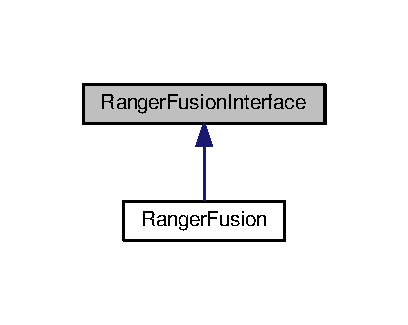
\includegraphics[width=196pt]{classRangerFusionInterface__inherit__graph}
\end{center}
\end{figure}
\subsection*{Public Member Functions}
\begin{DoxyCompactItemize}
\item 
virtual void {\bfseries set\+Rangers} (std\+::vector$<$ \hyperlink{classRangerInterface}{Ranger\+Interface} $\ast$ $>$ rangers)=0\hypertarget{classRangerFusionInterface_aea3d7cf254c0553e624306ca06d86120}{}\label{classRangerFusionInterface_aea3d7cf254c0553e624306ca06d86120}

\item 
virtual void {\bfseries set\+Cells} (std\+::vector$<$ \hyperlink{classCell}{Cell} $\ast$ $>$ cells)=0\hypertarget{classRangerFusionInterface_ab0b45c2c462124ce74d54eb226044beb}{}\label{classRangerFusionInterface_ab0b45c2c462124ce74d54eb226044beb}

\item 
virtual void {\bfseries grab\+And\+Fuse\+Data} ()=0\hypertarget{classRangerFusionInterface_ada6afdab2ce6d58a1bd0134f5e2be23f}{}\label{classRangerFusionInterface_ada6afdab2ce6d58a1bd0134f5e2be23f}

\item 
virtual std\+::vector$<$ std\+::vector$<$ double $>$ $>$ {\bfseries get\+Raw\+Range\+Data} ()=0\hypertarget{classRangerFusionInterface_a9d60ca5866261026b870d7c0171587f5}{}\label{classRangerFusionInterface_a9d60ca5866261026b870d7c0171587f5}

\end{DoxyCompactItemize}


The documentation for this class was generated from the following file\+:\begin{DoxyCompactItemize}
\item 
/home/ajal/git/pfms-\/2020a-\/ajalsingh/scratch/a2\+\_\+skeleton/rangerfusioninterface.\+h\end{DoxyCompactItemize}

\hypertarget{classRangerInterface}{}\section{Ranger\+Interface Class Reference}
\label{classRangerInterface}\index{Ranger\+Interface@{Ranger\+Interface}}


Inheritance diagram for Ranger\+Interface\+:\nopagebreak
\begin{figure}[H]
\begin{center}
\leavevmode
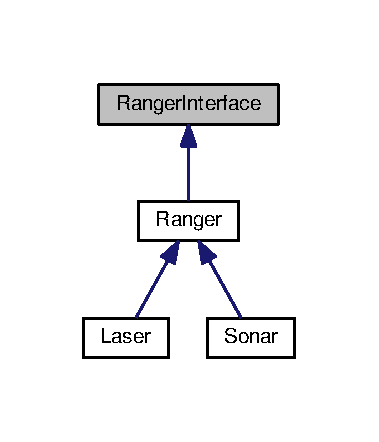
\includegraphics[width=182pt]{classRangerInterface__inherit__graph}
\end{center}
\end{figure}
\subsection*{Public Member Functions}
\begin{DoxyCompactItemize}
\item 
virtual std\+::vector$<$ double $>$ {\bfseries generate\+Data} ()=0\hypertarget{classRangerInterface_a969c670cadf55a15733809116dc305c8}{}\label{classRangerInterface_a969c670cadf55a15733809116dc305c8}

\item 
virtual unsigned int {\bfseries get\+Angular\+Resolution} (void)=0\hypertarget{classRangerInterface_a37d4f89daffa8b2708dfc11034893552}{}\label{classRangerInterface_a37d4f89daffa8b2708dfc11034893552}

\item 
virtual int {\bfseries get\+Offset} (void)=0\hypertarget{classRangerInterface_a8d77cf9d9b95fe8fb315931f2f278fec}{}\label{classRangerInterface_a8d77cf9d9b95fe8fb315931f2f278fec}

\item 
virtual unsigned int {\bfseries get\+Field\+Of\+View} (void)=0\hypertarget{classRangerInterface_a18716da6932402b8dda75f682be6f06c}{}\label{classRangerInterface_a18716da6932402b8dda75f682be6f06c}

\item 
virtual double {\bfseries get\+Max\+Range} (void)=0\hypertarget{classRangerInterface_a0bb29a41de5767c99081002c0590c186}{}\label{classRangerInterface_a0bb29a41de5767c99081002c0590c186}

\item 
virtual double {\bfseries get\+Min\+Range} (void)=0\hypertarget{classRangerInterface_ae6d501ddeeaad4a7b44d7d51ce64cb88}{}\label{classRangerInterface_ae6d501ddeeaad4a7b44d7d51ce64cb88}

\item 
virtual Sensing\+Method {\bfseries get\+Sensing\+Method} (void)=0\hypertarget{classRangerInterface_a6fdc6a8e9b3a4ebf0b1f5be3c607ef7d}{}\label{classRangerInterface_a6fdc6a8e9b3a4ebf0b1f5be3c607ef7d}

\item 
virtual bool {\bfseries set\+Angular\+Resolution} (unsigned int)=0\hypertarget{classRangerInterface_a313296ae5d13c6acce69caaf646ea66e}{}\label{classRangerInterface_a313296ae5d13c6acce69caaf646ea66e}

\item 
virtual bool {\bfseries set\+Offset} (int)=0\hypertarget{classRangerInterface_ae72584d83c94678d76f3fca20e432713}{}\label{classRangerInterface_ae72584d83c94678d76f3fca20e432713}

\item 
virtual bool {\bfseries set\+Field\+Of\+View} (unsigned int)=0\hypertarget{classRangerInterface_ad10f43a01e5285a654f09357028b1bb4}{}\label{classRangerInterface_ad10f43a01e5285a654f09357028b1bb4}

\end{DoxyCompactItemize}


The documentation for this class was generated from the following file\+:\begin{DoxyCompactItemize}
\item 
/home/ajal/git/pfms-\/2020a-\/ajalsingh/scratch/a2\+\_\+skeleton/rangerinterface.\+h\end{DoxyCompactItemize}

\hypertarget{classSonar}{}\section{Sonar Class Reference}
\label{classSonar}\index{Sonar@{Sonar}}


The \hyperlink{classSonar}{Sonar} class is a child class the \hyperlink{classRanger}{Ranger} Class Creates sonar objects of sensing method type C\+O\+NE.  




{\ttfamily \#include $<$sonar.\+h$>$}



Inheritance diagram for Sonar\+:\nopagebreak
\begin{figure}[H]
\begin{center}
\leavevmode
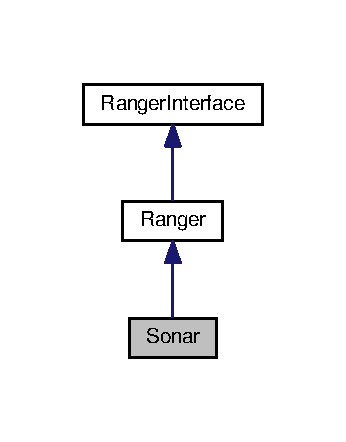
\includegraphics[width=166pt]{classSonar__inherit__graph}
\end{center}
\end{figure}


Collaboration diagram for Sonar\+:\nopagebreak
\begin{figure}[H]
\begin{center}
\leavevmode
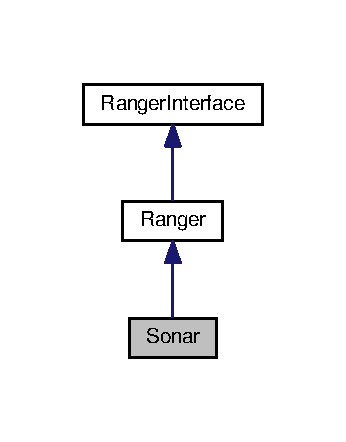
\includegraphics[width=166pt]{classSonar__coll__graph}
\end{center}
\end{figure}
\subsection*{Public Member Functions}
\begin{DoxyCompactItemize}
\item 
\hyperlink{classSonar_a71ef009d138f1e372fc35ca0cb6e85e2}{Sonar} ()
\begin{DoxyCompactList}\small\item\em \hyperlink{classSonar}{Sonar} default constructor. \end{DoxyCompactList}\item 
\hyperlink{classSonar_af344645fcd3ca9c20bdaf8342a87850b}{$\sim$\+Sonar} ()\hypertarget{classSonar_af344645fcd3ca9c20bdaf8342a87850b}{}\label{classSonar_af344645fcd3ca9c20bdaf8342a87850b}

\begin{DoxyCompactList}\small\item\em \hyperlink{classSonar}{Sonar} default destructor. \end{DoxyCompactList}\end{DoxyCompactItemize}
\subsection*{Additional Inherited Members}


\subsection{Detailed Description}
The \hyperlink{classSonar}{Sonar} class is a child class the \hyperlink{classRanger}{Ranger} Class Creates sonar objects of sensing method type C\+O\+NE. 

\begin{DoxyAuthor}{Author}
Ajal Singh 
\end{DoxyAuthor}
\begin{DoxyVersion}{Version}
1.\+0 
\end{DoxyVersion}
\begin{DoxyDate}{Date}
April 2020 
\end{DoxyDate}


\subsection{Constructor \& Destructor Documentation}
\index{Sonar@{Sonar}!Sonar@{Sonar}}
\index{Sonar@{Sonar}!Sonar@{Sonar}}
\subsubsection[{\texorpdfstring{Sonar()}{Sonar()}}]{\setlength{\rightskip}{0pt plus 5cm}Sonar\+::\+Sonar (
\begin{DoxyParamCaption}
{}
\end{DoxyParamCaption}
)}\hypertarget{classSonar_a71ef009d138f1e372fc35ca0cb6e85e2}{}\label{classSonar_a71ef009d138f1e372fc35ca0cb6e85e2}


\hyperlink{classSonar}{Sonar} default constructor. 

Default constructor sets the parameters to fixed params. Sets model, field of view, sensing method, angular resolution, max range and min range. 

The documentation for this class was generated from the following files\+:\begin{DoxyCompactItemize}
\item 
/home/ajal/git/pfms-\/2020a-\/ajalsingh/scratch/a2\+\_\+skeleton/\hyperlink{sonar_8h}{sonar.\+h}\item 
/home/ajal/git/pfms-\/2020a-\/ajalsingh/scratch/a2\+\_\+skeleton/sonar.\+cpp\end{DoxyCompactItemize}

\chapter{File Documentation}
\hypertarget{laser_8h}{}\section{/home/ajal/git/pfms-\/2020a-\/ajalsingh/scratch/a2\+\_\+skeleton/laser.h File Reference}
\label{laser_8h}\index{/home/ajal/git/pfms-\/2020a-\/ajalsingh/scratch/a2\+\_\+skeleton/laser.\+h@{/home/ajal/git/pfms-\/2020a-\/ajalsingh/scratch/a2\+\_\+skeleton/laser.\+h}}
{\ttfamily \#include \char`\"{}ranger.\+h\char`\"{}}\\*
Include dependency graph for laser.\+h\+:\nopagebreak
\begin{figure}[H]
\begin{center}
\leavevmode
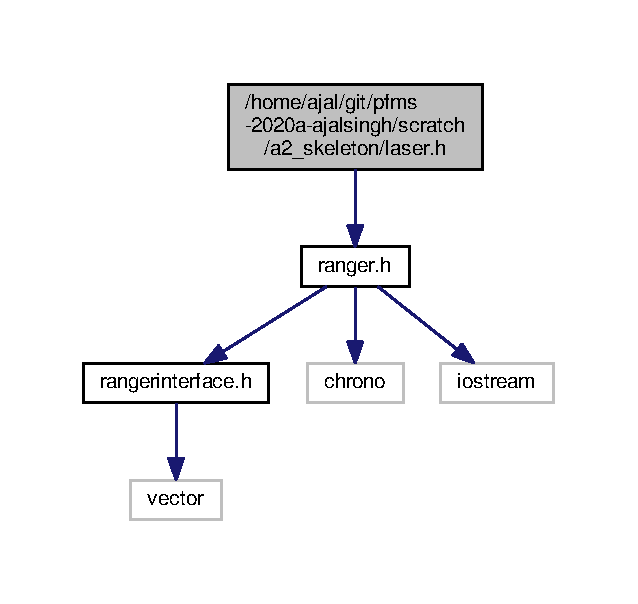
\includegraphics[width=306pt]{laser_8h__incl}
\end{center}
\end{figure}
This graph shows which files directly or indirectly include this file\+:\nopagebreak
\begin{figure}[H]
\begin{center}
\leavevmode
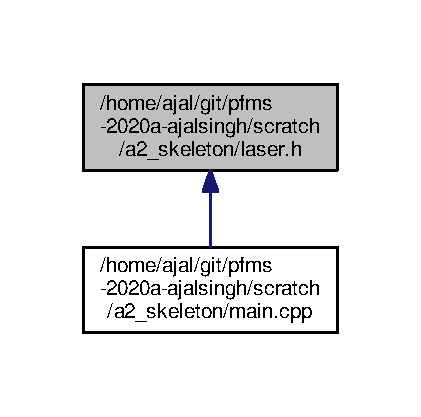
\includegraphics[width=202pt]{laser_8h__dep__incl}
\end{center}
\end{figure}
\subsection*{Classes}
\begin{DoxyCompactItemize}
\item 
class \hyperlink{classLaser}{Laser}
\begin{DoxyCompactList}\small\item\em The \hyperlink{classLaser}{Laser} class is a child class the \hyperlink{classRanger}{Ranger} Class. ~\newline
 This class creates lasers of sensing method type P\+O\+I\+NT. \end{DoxyCompactList}\end{DoxyCompactItemize}

\hypertarget{main_8cpp}{}\section{/home/ajal/git/pfms-\/2020a-\/ajalsingh/scratch/a2\+\_\+skeleton/main.cpp File Reference}
\label{main_8cpp}\index{/home/ajal/git/pfms-\/2020a-\/ajalsingh/scratch/a2\+\_\+skeleton/main.\+cpp@{/home/ajal/git/pfms-\/2020a-\/ajalsingh/scratch/a2\+\_\+skeleton/main.\+cpp}}


main  


{\ttfamily \#include \char`\"{}laser.\+h\char`\"{}}\\*
{\ttfamily \#include \char`\"{}sonar.\+h\char`\"{}}\\*
{\ttfamily \#include \char`\"{}rangerfusion.\+h\char`\"{}}\\*
{\ttfamily \#include \char`\"{}cell.\+h\char`\"{}}\\*
{\ttfamily \#include $<$iostream$>$}\\*
{\ttfamily \#include $<$thread$>$}\\*
{\ttfamily \#include $<$chrono$>$}\\*
{\ttfamily \#include $<$iomanip$>$}\\*
{\ttfamily \#include $<$random$>$}\\*
Include dependency graph for main.\+cpp\+:\nopagebreak
\begin{figure}[H]
\begin{center}
\leavevmode
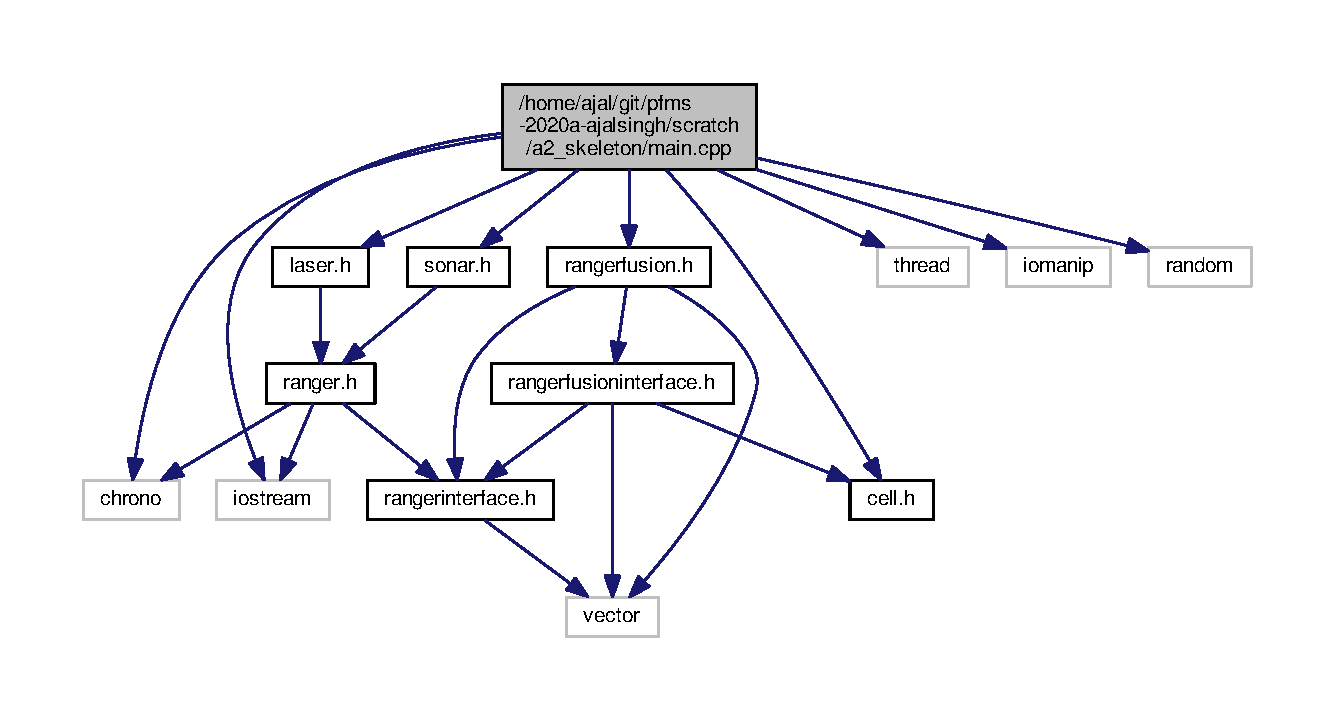
\includegraphics[width=350pt]{main_8cpp__incl}
\end{center}
\end{figure}
\subsection*{Functions}
\begin{DoxyCompactItemize}
\item 
void \hyperlink{main_8cpp_a45dfa865ea2a3e47b592321e9e129300}{get\+Fixed\+Params} (const std\+::vector$<$ \hyperlink{classRanger}{Ranger} $\ast$ $>$ rangers)
\begin{DoxyCompactList}\small\item\em Prints Fixed Params for Rangers on console. \end{DoxyCompactList}\item 
void \hyperlink{main_8cpp_a4df4a53a2f8566f3a0138e219a652ba8}{get\+Raw\+Data} (const std\+::vector$<$ std\+::vector$<$ double $>$$>$ raw)
\begin{DoxyCompactList}\small\item\em Prints Raw data to console. \end{DoxyCompactList}\item 
void \hyperlink{main_8cpp_a335ffcf745b11f0771ec1e7aee0b1722}{ranger\+Configuration} (std\+::vector$<$ \hyperlink{classRanger}{Ranger} $\ast$ $>$ \&rangers)
\begin{DoxyCompactList}\small\item\em Configures ranger params according to type and user\textquotesingle{}s specifications. \end{DoxyCompactList}\item 
void \hyperlink{main_8cpp_a5c7c526411e4f9aaad664f1f41ad5ac4}{cell\+Configuration} (std\+::vector$<$ \hyperlink{classCell}{Cell} $\ast$ $>$ \&cells, std\+::vector$<$ \hyperlink{classRanger}{Ranger} $\ast$ $>$ \&rangers)
\begin{DoxyCompactList}\small\item\em Creates number of cells specified by user. ~\newline
 Randomly set centre location on grid based on ranger max distance. \end{DoxyCompactList}\item 
void \hyperlink{main_8cpp_a0328635da38f7f37dd18b0e886e1dbc1}{print\+Cell\+Locations} (const std\+::vector$<$ \hyperlink{classCell}{Cell} $\ast$ $>$ cells)
\begin{DoxyCompactList}\small\item\em Prints coordinates of cell centre. \end{DoxyCompactList}\item 
int \hyperlink{main_8cpp_ae66f6b31b5ad750f1fe042a706a4e3d4}{main} ()
\begin{DoxyCompactList}\small\item\em Main Function creates lasers, sonar and \hyperlink{classRangerFusion}{Ranger\+Fusion} objects and stores them in corresponding vectors ~\newline
 Allows the user to configure rangers and cells and displays params/cell locations to console. ~\newline
 Passes cells and rangers to fusion class for processing. ~\newline
 Get updates cell state data and continuously print States to console ~\newline
 \hyperlink{classRanger}{Ranger} data is continuously passed to fusion class and cell state is continuously returned. \end{DoxyCompactList}\end{DoxyCompactItemize}
\subsection*{Variables}
\begin{DoxyCompactItemize}
\item 
int \hyperlink{main_8cpp_a1447ad288a0a73454510f5777bdc3ed1}{seed} = std\+::chrono\+::system\+\_\+clock\+::now().time\+\_\+since\+\_\+epoch().count()\hypertarget{main_8cpp_a1447ad288a0a73454510f5777bdc3ed1}{}\label{main_8cpp_a1447ad288a0a73454510f5777bdc3ed1}

\begin{DoxyCompactList}\small\item\em Holds the seed used in random number generation. \end{DoxyCompactList}\item 
int \hyperlink{main_8cpp_a4990e0064e9ccc91095d3aa899494869}{fusion\+\_\+count} =1\hypertarget{main_8cpp_a4990e0064e9ccc91095d3aa899494869}{}\label{main_8cpp_a4990e0064e9ccc91095d3aa899494869}

\begin{DoxyCompactList}\small\item\em The number of fusions that have occured. \end{DoxyCompactList}\end{DoxyCompactItemize}


\subsection{Detailed Description}
main 

\begin{DoxyAuthor}{Author}
Ajal Singh 
\end{DoxyAuthor}
\begin{DoxyVersion}{Version}
1.\+0 
\end{DoxyVersion}
\begin{DoxyDate}{Date}
April 2020 
\end{DoxyDate}


\subsection{Function Documentation}
\index{main.\+cpp@{main.\+cpp}!cell\+Configuration@{cell\+Configuration}}
\index{cell\+Configuration@{cell\+Configuration}!main.\+cpp@{main.\+cpp}}
\subsubsection[{\texorpdfstring{cell\+Configuration(std\+::vector$<$ Cell $\ast$ $>$ \&cells, std\+::vector$<$ Ranger $\ast$ $>$ \&rangers)}{cellConfiguration(std::vector< Cell * > &cells, std::vector< Ranger * > &rangers)}}]{\setlength{\rightskip}{0pt plus 5cm}void cell\+Configuration (
\begin{DoxyParamCaption}
\item[{std\+::vector$<$ {\bf Cell} $\ast$ $>$ \&}]{cells, }
\item[{std\+::vector$<$ {\bf Ranger} $\ast$ $>$ \&}]{rangers}
\end{DoxyParamCaption}
)}\hypertarget{main_8cpp_a5c7c526411e4f9aaad664f1f41ad5ac4}{}\label{main_8cpp_a5c7c526411e4f9aaad664f1f41ad5ac4}


Creates number of cells specified by user. ~\newline
 Randomly set centre location on grid based on ranger max distance. 


\begin{DoxyParams}{Parameters}
{\em cells} & -\/ vector of pointers \\
\hline
{\em rangers} & -\/ vector of pointers \\
\hline
\end{DoxyParams}
\index{main.\+cpp@{main.\+cpp}!get\+Fixed\+Params@{get\+Fixed\+Params}}
\index{get\+Fixed\+Params@{get\+Fixed\+Params}!main.\+cpp@{main.\+cpp}}
\subsubsection[{\texorpdfstring{get\+Fixed\+Params(const std\+::vector$<$ Ranger $\ast$ $>$ rangers)}{getFixedParams(const std::vector< Ranger * > rangers)}}]{\setlength{\rightskip}{0pt plus 5cm}void get\+Fixed\+Params (
\begin{DoxyParamCaption}
\item[{const std\+::vector$<$ {\bf Ranger} $\ast$ $>$}]{rangers}
\end{DoxyParamCaption}
)}\hypertarget{main_8cpp_a45dfa865ea2a3e47b592321e9e129300}{}\label{main_8cpp_a45dfa865ea2a3e47b592321e9e129300}


Prints Fixed Params for Rangers on console. 


\begin{DoxyParams}{Parameters}
{\em rangers} & -\/ vector of pointers \\
\hline
\end{DoxyParams}
\index{main.\+cpp@{main.\+cpp}!get\+Raw\+Data@{get\+Raw\+Data}}
\index{get\+Raw\+Data@{get\+Raw\+Data}!main.\+cpp@{main.\+cpp}}
\subsubsection[{\texorpdfstring{get\+Raw\+Data(const std\+::vector$<$ std\+::vector$<$ double $>$$>$ raw)}{getRawData(const std::vector< std::vector< double >> raw)}}]{\setlength{\rightskip}{0pt plus 5cm}void get\+Raw\+Data (
\begin{DoxyParamCaption}
\item[{const std\+::vector$<$ std\+::vector$<$ double $>$$>$}]{raw}
\end{DoxyParamCaption}
)}\hypertarget{main_8cpp_a4df4a53a2f8566f3a0138e219a652ba8}{}\label{main_8cpp_a4df4a53a2f8566f3a0138e219a652ba8}


Prints Raw data to console. 


\begin{DoxyParams}{Parameters}
{\em raw} & Data -\/ vector of vector doubles \\
\hline
\end{DoxyParams}
\index{main.\+cpp@{main.\+cpp}!main@{main}}
\index{main@{main}!main.\+cpp@{main.\+cpp}}
\subsubsection[{\texorpdfstring{main()}{main()}}]{\setlength{\rightskip}{0pt plus 5cm}int main (
\begin{DoxyParamCaption}
{}
\end{DoxyParamCaption}
)}\hypertarget{main_8cpp_ae66f6b31b5ad750f1fe042a706a4e3d4}{}\label{main_8cpp_ae66f6b31b5ad750f1fe042a706a4e3d4}


Main Function creates lasers, sonar and \hyperlink{classRangerFusion}{Ranger\+Fusion} objects and stores them in corresponding vectors ~\newline
 Allows the user to configure rangers and cells and displays params/cell locations to console. ~\newline
 Passes cells and rangers to fusion class for processing. ~\newline
 Get updates cell state data and continuously print States to console ~\newline
 \hyperlink{classRanger}{Ranger} data is continuously passed to fusion class and cell state is continuously returned. 

\begin{DoxyNote}{Note}
User must manually terminate program. 
\end{DoxyNote}
\index{main.\+cpp@{main.\+cpp}!print\+Cell\+Locations@{print\+Cell\+Locations}}
\index{print\+Cell\+Locations@{print\+Cell\+Locations}!main.\+cpp@{main.\+cpp}}
\subsubsection[{\texorpdfstring{print\+Cell\+Locations(const std\+::vector$<$ Cell $\ast$ $>$ cells)}{printCellLocations(const std::vector< Cell * > cells)}}]{\setlength{\rightskip}{0pt plus 5cm}void print\+Cell\+Locations (
\begin{DoxyParamCaption}
\item[{const std\+::vector$<$ {\bf Cell} $\ast$ $>$}]{cells}
\end{DoxyParamCaption}
)}\hypertarget{main_8cpp_a0328635da38f7f37dd18b0e886e1dbc1}{}\label{main_8cpp_a0328635da38f7f37dd18b0e886e1dbc1}


Prints coordinates of cell centre. 


\begin{DoxyParams}{Parameters}
{\em cells} & -\/ vector of pointers \\
\hline
\end{DoxyParams}
\index{main.\+cpp@{main.\+cpp}!ranger\+Configuration@{ranger\+Configuration}}
\index{ranger\+Configuration@{ranger\+Configuration}!main.\+cpp@{main.\+cpp}}
\subsubsection[{\texorpdfstring{ranger\+Configuration(std\+::vector$<$ Ranger $\ast$ $>$ \&rangers)}{rangerConfiguration(std::vector< Ranger * > &rangers)}}]{\setlength{\rightskip}{0pt plus 5cm}void ranger\+Configuration (
\begin{DoxyParamCaption}
\item[{std\+::vector$<$ {\bf Ranger} $\ast$ $>$ \&}]{rangers}
\end{DoxyParamCaption}
)}\hypertarget{main_8cpp_a335ffcf745b11f0771ec1e7aee0b1722}{}\label{main_8cpp_a335ffcf745b11f0771ec1e7aee0b1722}


Configures ranger params according to type and user\textquotesingle{}s specifications. 


\begin{DoxyParams}{Parameters}
{\em rangers} & -\/ vector of pointers \\
\hline
\end{DoxyParams}

\hypertarget{ranger_8h}{}\section{/home/ajal/git/pfms-\/2020a-\/ajalsingh/scratch/a2\+\_\+skeleton/ranger.h File Reference}
\label{ranger_8h}\index{/home/ajal/git/pfms-\/2020a-\/ajalsingh/scratch/a2\+\_\+skeleton/ranger.\+h@{/home/ajal/git/pfms-\/2020a-\/ajalsingh/scratch/a2\+\_\+skeleton/ranger.\+h}}
{\ttfamily \#include \char`\"{}rangerinterface.\+h\char`\"{}}\\*
{\ttfamily \#include $<$chrono$>$}\\*
{\ttfamily \#include $<$iostream$>$}\\*
Include dependency graph for ranger.\+h\+:\nopagebreak
\begin{figure}[H]
\begin{center}
\leavevmode
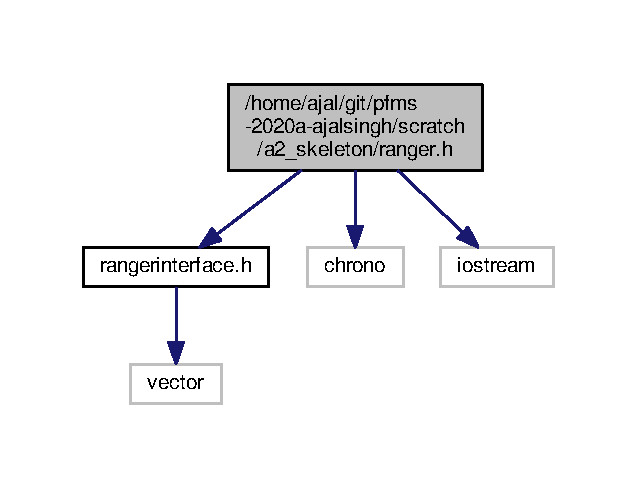
\includegraphics[width=306pt]{ranger_8h__incl}
\end{center}
\end{figure}
This graph shows which files directly or indirectly include this file\+:\nopagebreak
\begin{figure}[H]
\begin{center}
\leavevmode
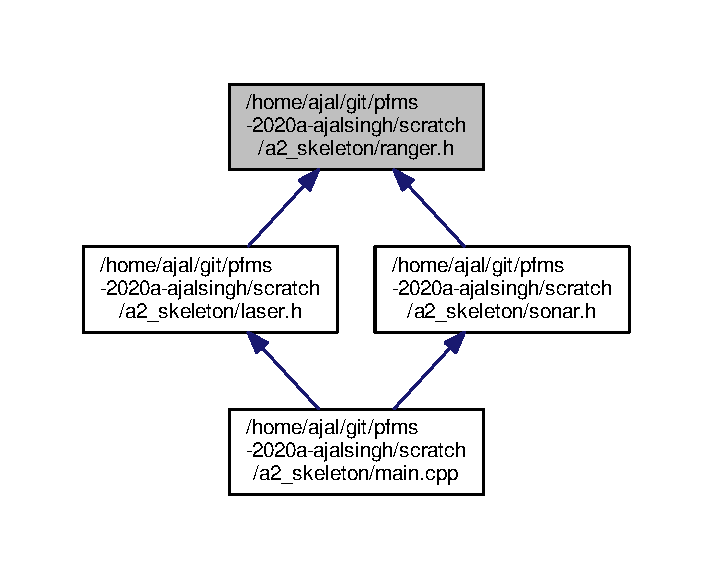
\includegraphics[width=342pt]{ranger_8h__dep__incl}
\end{center}
\end{figure}
\subsection*{Classes}
\begin{DoxyCompactItemize}
\item 
class \hyperlink{classRanger}{Ranger}
\begin{DoxyCompactList}\small\item\em This class inherits methods from abstract class \hyperlink{classRangerInterface}{Ranger\+Interface} ~\newline
 This class is the base class to sensor classes (laser/sonar) \end{DoxyCompactList}\end{DoxyCompactItemize}

\hypertarget{rangerfusion_8h}{}\section{/home/ajal/git/pfms-\/2020a-\/ajalsingh/scratch/a2\+\_\+skeleton/rangerfusion.h File Reference}
\label{rangerfusion_8h}\index{/home/ajal/git/pfms-\/2020a-\/ajalsingh/scratch/a2\+\_\+skeleton/rangerfusion.\+h@{/home/ajal/git/pfms-\/2020a-\/ajalsingh/scratch/a2\+\_\+skeleton/rangerfusion.\+h}}
{\ttfamily \#include $<$vector$>$}\\*
{\ttfamily \#include \char`\"{}rangerfusioninterface.\+h\char`\"{}}\\*
{\ttfamily \#include \char`\"{}rangerinterface.\+h\char`\"{}}\\*
Include dependency graph for rangerfusion.\+h\+:\nopagebreak
\begin{figure}[H]
\begin{center}
\leavevmode
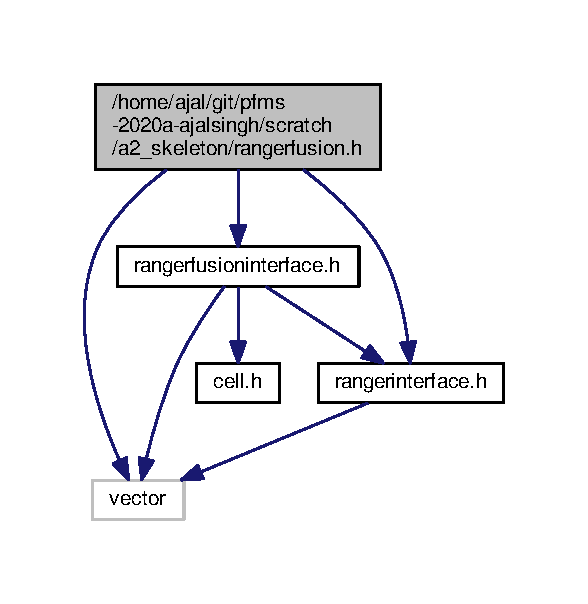
\includegraphics[width=282pt]{rangerfusion_8h__incl}
\end{center}
\end{figure}
This graph shows which files directly or indirectly include this file\+:\nopagebreak
\begin{figure}[H]
\begin{center}
\leavevmode
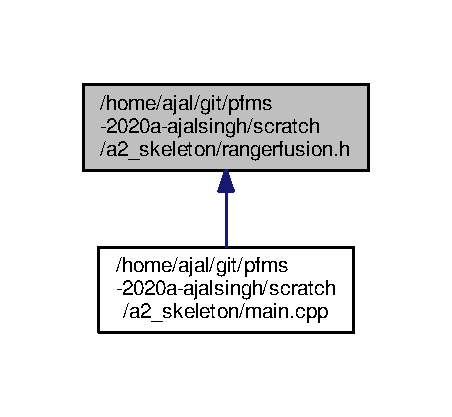
\includegraphics[width=217pt]{rangerfusion_8h__dep__incl}
\end{center}
\end{figure}
\subsection*{Classes}
\begin{DoxyCompactItemize}
\item 
struct \hyperlink{structPoint}{Point}
\begin{DoxyCompactList}\small\item\em The \hyperlink{structPoint}{Point} struct. Creates points with x and y coordinates. \end{DoxyCompactList}\item 
class \hyperlink{classRangerFusion}{Ranger\+Fusion}
\begin{DoxyCompactList}\small\item\em The \hyperlink{classRangerFusion}{Ranger\+Fusion} class is a child of abstract class \hyperlink{classRangerFusionInterface}{Ranger\+Fusion\+Interface} Accepts cells and rangers and fuses the data. Checks if the ranger data occupies a cell, or passes through the cell (free). \hyperlink{classCell}{Cell} state is then updated. \end{DoxyCompactList}\end{DoxyCompactItemize}

\hypertarget{sonar_8h}{}\section{/home/ajal/git/pfms-\/2020a-\/ajalsingh/scratch/a2\+\_\+skeleton/sonar.h File Reference}
\label{sonar_8h}\index{/home/ajal/git/pfms-\/2020a-\/ajalsingh/scratch/a2\+\_\+skeleton/sonar.\+h@{/home/ajal/git/pfms-\/2020a-\/ajalsingh/scratch/a2\+\_\+skeleton/sonar.\+h}}
{\ttfamily \#include \char`\"{}ranger.\+h\char`\"{}}\\*
Include dependency graph for sonar.\+h\+:\nopagebreak
\begin{figure}[H]
\begin{center}
\leavevmode
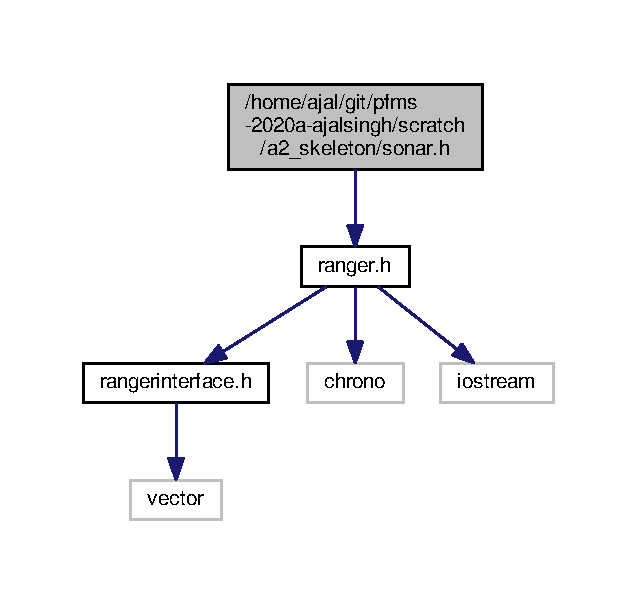
\includegraphics[width=306pt]{sonar_8h__incl}
\end{center}
\end{figure}
This graph shows which files directly or indirectly include this file\+:\nopagebreak
\begin{figure}[H]
\begin{center}
\leavevmode
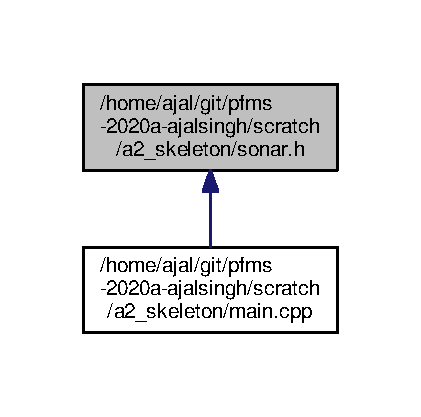
\includegraphics[width=202pt]{sonar_8h__dep__incl}
\end{center}
\end{figure}
\subsection*{Classes}
\begin{DoxyCompactItemize}
\item 
class \hyperlink{classSonar}{Sonar}
\begin{DoxyCompactList}\small\item\em The \hyperlink{classSonar}{Sonar} class is a child class the \hyperlink{classRanger}{Ranger} Class Creates sonar objects of sensing method type C\+O\+NE. \end{DoxyCompactList}\end{DoxyCompactItemize}

%--- End generated contents ---

% Index
\backmatter
\newpage
\phantomsection
\clearemptydoublepage
\addcontentsline{toc}{chapter}{Index}
\printindex

\end{document}
